
\documentclass[grid,avery5371,landscape]{flashcards}

\usepackage[T1]{fontenc}
\usepackage[sfdefault,semibold,scaled=.85]{FiraSans}
\usepackage{graphicx}
\usepackage{newtxsf}
\usepackage{xcolor}
\usepackage{calc}
\usepackage{geometry}
\usepackage{enumitem}

\geometry{a4paper,portrait}

\renewcommand{\cardpaper}{a4paper}
\renewcommand{\cardpapermode}{landscape}
\renewcommand{\cardrows}{4}
\renewcommand{\cardcolumns}{2}
\setlength{\cardheight}{54mm-2\fboxrule}
\setlength{\cardwidth}{85mm-2\fboxrule}
\setlength{\topoffset}{0mm}
\setlength{\oddoffset}{0.0mm}
\setlength{\evenoffset}{0.0mm}
\setlength{\cardmargin}{2.5mm}
\setlength{\fboxrule}{2.5mm}


\cardfrontstyle[\raggedright\large\color{black}]{headings}
\cardbackstyle[\raggedright\small\color{black}]{plain}
\cardfrontheadstyle[\small\color{black}]{left}
\newcounter{nocarte}
\newcommand{\categ}[1]{%
  \def\@categ{#1}%
  \setcounter{nocarte}{0}%
}
\cardfrontfoot{\textcolor{black}{\@categ --\refstepcounter{nocarte} \thenocarte}}
\cardfrontfootstyle[\small]{right}


\setlist[itemize]{label=$\bullet$,labelindent=0em,labelsep=1ex,leftmargin=*,labelwidth=1em,itemsep=0mm}

\newcommand{\source}[1]{%
  \medskip
  \itshape%
   ~ \hfill Réf. : #1}

\begin{document}


\color[HTML]{01DF01}
\categ{CE-CP-REG}
\begin{flashcard}[bilan]{
 Qu'est-ce qu'un infarctus du myocarde (IdM) ? Quels en sont les signes ?   }
   Un infarctus est nécrose du muscle cardiaque liée à l'occlusion complète des artères qui le vascularisent.  Il s'agit d'une urgence vitale circulatoire. 
   \begin{itemize}        
\item douleur retro-sternal conscritive avec possible irradiation dans la mâchoire et le bras gauche       
\item intensitée très forte (sensation de mort imminente)        
\item ne cède pas au repos ($>$15 minutes)       
 \item ne cède pas à la prise de vasodilatateurs  
 \end{itemize}
  \source{Diapo for CE }
\end{flashcard}


\color[HTML]{01DF01}
\categ{CE-CP-REG}
\begin{flashcard}[bilan]{
 Quels sont les facteurs de risque d'un infarctus du myocarde (IdM) ?   }
  Les facteurs de risque, pour les pathologies coronariennes telles que l'IdM, sont : âge, antécédents familiaux, diabète, cholestérol, hypertension, tabagisme, cocaïne.
  \source{Diapo for CE }
\end{flashcard}


\color[HTML]{01DF01}
\categ{CE-CP-REG}
\begin{flashcard}[CAT]{
 Quelle CAT face à un infarctus du myocarde (IdM) ?   }
  La position d'attente est allongée stricte. \\    Il s'agit d'une urgence vitale nécessitant un contact à la régulation immédiat. \\   L'équipe doit se préparer à effectuer une réanimation cardio-pulmonaire.
  \source{Diapo for CE }
\end{flashcard}


\color[HTML]{01DF01}
\categ{CE-CP-REG}
\begin{flashcard}[bilan]{
 Qu'est-ce qu'une crise d'angor ? Quelle en sont les signes ?   }
  Une crise d'angor est un réduction (sans obstruction) des vaisseaux irriguant le coeur (les coronaires).  Il s'agit d'une urgence vitale circulatoire.
   \begin{itemize}
       \item douleur retro-sternal conscrictive avec possible irradiation dans la mâchoire et le bras gauche
       \item apparue souvent à l'effort ou au stress
       \item cède au repos ($<$5 minutes)
       \item cède à la prise de vasodilatateurs
   \end{itemize}
  \source{Diapo for CE }
\end{flashcard}


\color[HTML]{01DF01}
\categ{CE-CP-REG}
\begin{flashcard}[bilan]{
 Quels sont les facteurs de risque d'une crise d'angor ?   }
  Les facteurs de risque, pour les pathologies coronariennes telles que la crise d'angor, sont : âge, antécédents familiaux, diabète, cholestérol, hypertension, tabagisme, cocaïne.
  \source{Diapo for CE }
\end{flashcard}


\color[HTML]{01DF01}
\categ{CE-CP-REG}
\begin{flashcard}[CAT]{
 Quelle CAT face à une crise d'angor ?   }
  La position d'attente est allongée stricte. \\
   Il s'agit d'une urgence vitale nécessitant un contact à la régulation immédiat.\\
   L'équipe doit se préparer à effectuer une réanimation cardio-pulmonaire.
  \source{Diapo for CE }
\end{flashcard}


\color[HTML]{01DF01}
\categ{CE-CP-REG}
\begin{flashcard}[bilan]{
 Qu'est-ce qu'une péricardite ? Quelle en sont les signes ?   }
  Une péricardite est une inflammation de la membre entourant le coeur. Il s'agit d'une urgence vitale circulatoire.
   \begin{itemize}
       \item douleur précodirale conscrictive avec possible irradiation dans la mâchoire et le bras gauche
       \item fréquence respiratoire élevée
       \item douleur amplifiée à l'inspiration
       \item douleur atténuée lorsque la victime est penchée en avant
   \end{itemize}
  \source{Diapo for CE }
\end{flashcard}


\color[HTML]{01DF01}
\categ{CE-CP-REG}
\begin{flashcard}[CAT]{
 Quelle CAT face à un péricardite ?   }
  La position d'attente est allongée stricte. \\
   Il s'agit d'une urgence vitale nécessitant un contact à la régulation immédiat.\\
   L'équipe doit se préparer à effectuer une réanimation cardio-pulmonaire.
  \source{Diapo for CE }
\end{flashcard}


\color[HTML]{01DF01}
\categ{CE-CP-REG}
\begin{flashcard}[bilan]{
 Quels sont les facteurs de risque d'une péricardite ?   }
  Les facteurs de risques sont :
   \begin{itemize}
       \item infection récente
       \item cancer, radiothérapie
       \item insuffisance rénale
       \item maladie systémique
       \item infarctus ou chirurgie cardiaque récente
       \item prise de médicament
       \item antécédent de péricardite
   \end{itemize}
   La péricardite concerne usuellement des sujets jeunes.
  \source{Diapo for CE }
\end{flashcard}


\color[HTML]{01DF01}
\categ{CE-CP-REG}
\begin{flashcard}[bilan]{
 Qu'est-ce qu'une dissection aortique ? Quelle en sont les signes ?   }
  Une dissection aortique est une rupture de la membre de l'aorte dans la longueur sous l'effet de la pression artérielle.
   \begin{itemize}
       \item douleur précodirale conscrictive avec possible irradiation dans le dos
       \item survenue brutale
       \item asymétrie circulatoire supérieur : écart de plus de 20mmHg de PA entre les deux bras, pouls présent que d'un côté, etc.
       \item douleur très intense, possiblement mouvante
   \end{itemize}
  \source{Diapo for CE }
\end{flashcard}


\color[HTML]{01DF01}
\categ{CE-CP-REG}
\begin{flashcard}[bilan]{
 Quels sont les facteurs de risque d'une dissection aortique  ?   }
  Les facteurs de risques sont :
   \begin{itemize}
       \item hypertension, 
       \item maladie congénitale, m
       \item maladie inflammatoire aortique, 
       \item maladie systémique, 
       \item grossesse (en cours ou récente), 
       \item athérosclérose (maladie des vaisseaux sanguins),
       \item tabagisme.
   \end{itemize}
  \source{Diapo for CE }
\end{flashcard}


\color[HTML]{01DF01}
\categ{CE-CP-REG}
\begin{flashcard}[CAT]{
 Quelle CAT face à une dissection aortique ?   }
  La position d'attente est allongée stricte. \\
   Il s'agit d'une urgence vitale nécessitant un contact à la régulation immédiat.\\
   L'équipe doit se préparer à effectuer une réanimation cardio-pulmonaire.
  \source{Diapo for CE }
\end{flashcard}


\color[HTML]{01DF01}
\categ{CE-CP-REG}
\begin{flashcard}[bilan]{
 Qu'est-ce qu'un accident vasculaire cérébral? Quels sont les signes ?   }
  Un AVC est une perte soudaine de la fonction cérébrale provoqué par un arrêt de la circulation sanguine dans le cerveau. Il y a les AVC ischémique (les plus courants) et les AVC hémorragiques (plus rares). \\
    Les signes sont FAST : déformation du visage (Face) gonfler les joues-, difficultés à lever les deux bras parallèlement (Arm), difficulté délocution (Speech), la durée/heure de survenu (Time).
  \source{Diapo for CE }
\end{flashcard}


\color[HTML]{01DF01}
\categ{CE-CP-REG}
\begin{flashcard}[CAT]{
 Quelle CAT face à un AVC ?   }
  Un AVC est une urgence vitale nécessitant un appel immédiat à la régulation. \\
    Les informations complémentaires sont : lheure de survenue de lépisode, les antécédents, les facteurs déclenchant, traitement en cours (anticoagulant), si la victime est grabataire, hypoglycémie, et des contre-indications à une IRM (pacemaker, prothèse, stems, etc.).
  \source{Diapo for CE }
\end{flashcard}


\color[HTML]{01DF01}
\categ{CE-CP-REG}
\begin{flashcard}[bilan]{
 Qu'est-ce qu'une méningite? Quels sont les signes ?   }
  Une méningite est une inflammation, d' origine virale ou bactérienne, de la membrane qui entoure le système nerveux.  Elle apparaît spontanément ou à la suite d'actes chirurgicaux ou de traumatismes crâniens. \\
    Les signes principaux sont : une raideur de la nuque [demander de toucher la poitrine avec le menton], nausées/vomissements en jet, céphalées violentes, photophobie, fièvre. Les signes complémentaires sont : le contact avec une personne atteinte, allergies, position en chien de fusil, \textit{purpura fulminans} (tâche en lie de vin).
  \source{Diapo for CE }
\end{flashcard}


\color[HTML]{01DF01}
\categ{CE-CP-REG}
\begin{flashcard}[CAT]{
 Quelle CAT face à une méningite ?   }
  La méningite est une maladie très contagieuse : lengagement doit être minimal (1 secouriste si possible) avec un équipement de protection individuel. Poser un masque chirurgical à la victime et à ses proches. 
  \source{Diapo for CE }
\end{flashcard}


\color[HTML]{01DF01}
\categ{CE-CP-REG}
\begin{flashcard}[bilan]{
 Qu'est-ce qu'une crise convulsive ? Quels sont les signes ?   }
  Une crise convulsive est a survenue brutale et inopinée de spasmes musculaires involontaires pouvant concerner un muscle isolément, mais aussi l'ensemble du corps.
  \source{Diapo for CE }
\end{flashcard}


\color[HTML]{01DF01}
\categ{CE-CP-REG}
\begin{flashcard}[CAT]{
 Quelle CAT face à une crise convulsive ?   }
  Protéger la victime en la laissant convulser : au sol, loin des meubles, etc. \\
Les informations complémentaires sont : lheure de survenue de lépisode, les antécédents, les facteurs déclenchant (fatigue, stimulation lumineuse, prise d'alcool oude stupéfiants) et les traitements en cours (insuline, etc.).
  \source{Diapo for CE }
\end{flashcard}


\color[HTML]{01DF01}
\categ{CE-CP-REG}
\begin{flashcard}[bilan]{
 Qu'est-ce que l'asthme? Quels sont les signes ?   }
  L'asthme est une diminution du diamètre des bronches. Il peut être allergique ou non.  \\
    Outre les signes d'une détresse respiratoire, l'asthme s'identifie par un sifflement et un effort à l'expiration.
  \source{Diapo for CE }
\end{flashcard}


\color[HTML]{01DF01}
\categ{CE-CP-REG}
\begin{flashcard}[CAT]{
 Quelle CAT face à une crisme d'asthme ?   }
  Rassurer la victime et l'aider si possible à prendre son traitement (vaporisation en inspirant, garder sa respiration qq secondes pour que la dilatation s'opère, expiration).
 \\
    En complément, identifier le facteur déclenchant et caractériser la crise (durée, prise de traitement, efficacité).
  \source{Diapo for CE }
\end{flashcard}


\color[HTML]{01DF01}
\categ{CE-CP-REG}
\begin{flashcard}[bilan]{
 Qu'est-ce que l'IRC? Quels sont les signes ?   }
  L'insuffisance respiratoire chronique est une patholgie (de type BPCO) où le corps de la victime s'est adaptée à fonctionner avec une saturation en oxygène diminuée. Les patients en IRC ont souvent de l'oxygène à domicile. \\ Une victime IRC en détresse présente une saturation inférieure à sa saturation usuelle, est agitée ou attente de somnolence.
  \source{Diapo for CE }
\end{flashcard}


\color[HTML]{01DF01}
\categ{CE-CP-REG}
\begin{flashcard}[CAT]{
 Quelle CAT face à un IRC ?   }
  Il faut identifier les circonstances de l'appel, le facteur déclenchant, interroger sur la prise d'un traitement et identifier le débit usuel de la victime.\\ La prise en charge consiste à administrer de l'oxygène à la victime à un débit 1 à 2$L/min$ supérieur au débit usuel pour restaurer une saturation entre 84\% et 89\%.
  \source{Diapo for CE }
\end{flashcard}


\color[HTML]{01DF01}
\categ{CE-CP-REG}
\begin{flashcard}[bilan]{
 Qu'est-ce qu'un pneumothorax ? Quels sont les signes ?   }
  Un pneumothorax se caractérise par la présence dair dans la cavité pleurale. Il peut être d'origine spontanée ou traumatique.  \\
    La victime présente une vive douleur à la poitrine d'apparition brutale, des difficultés respiratoires (d'apparition brutale) et une toux persistante.
  \source{Diapo for CE }
\end{flashcard}


\color[HTML]{01DF01}
\categ{CE-CP-REG}
\begin{flashcard}[CAT]{
 Quelle CAT face à un pneumothorax ?   }
  Il faut identifier le facteur déclenchant et les conditions d'apparition (brutale ?). La position d'attente est assise.
  \source{Diapo for CE }
\end{flashcard}


\color[HTML]{01DF01}
\categ{CE-CP-REG}
\begin{flashcard}[bilan]{
 Qu'est-ce qu'un hémothorax ? Quels sont les signes ?   }
  Un hémothorax se caractérise par un épanchement de sang dans la cavité pleurale. L'hémothorax est d'origine traumatique.  \\
    Les signes sont : douleurs localisés au niveau du thorax, toux sèche (aux changements de positions), essoufflement possible, perte d'appétit, amaigrissement, fatigue importante, hyperthermie en cas d'infection.
  \source{Diapo for CE }
\end{flashcard}


\color[HTML]{01DF01}
\categ{CE-CP-REG}
\begin{flashcard}[CAT]{
 Quelle CAT face à un pneumothorax ?   }
  La position d'attente est assise (A VERIFIER).
    Un hémothorax nécessite un appel à la régulation.
  \source{Diapo for CE }
\end{flashcard}


\color[HTML]{01DF01}
\categ{CE-CP-REG}
\begin{flashcard}[bilan]{
 Qu'est-ce qu'une embolie pulmonaire ? Quels sont les signes ?   }
  Une embolie pulmonaire est lobstruction dune artère irriguant un poumon par un caillot ambulant (thrombus). Il sagit dune complication majeure dune phlébite (caillot bloquant une veine, souvent dans un membre inférieur). \\ Les signes sont : douleurs basi-thoracique, douleur de survenue brutale, difficultés respiratoires, augmentation de la fréquence respiratoire, angoisse, douleur et ou raideur du mollet.
  \source{Diapo for CE }
\end{flashcard}


\color[HTML]{01DF01}
\categ{CE-CP-REG}
\begin{flashcard}[bilan]{
 Quels sont les facteurs d'une embolie pulmonaire ?   }
  Les facteurs de risques sont :
   \begin{itemize}
       \item immobilisation prolongée, 
       \item traumatisme du bassin ou des membres inférieurs.     
       \item opération chirurgicale (dans les 3 derniers mois), 
       \item antécédent dEP ou de trouble de la coagulation, 
       \item insuffisance cardiaque congestive, BPCO, obésité, cancer, 
       \item grossesse (actuelle ou récente), contraception orale, 
       \item tabagisme
   \end{itemize}
  \source{Diapo for CE }
\end{flashcard}


\color[HTML]{01DF01}
\categ{CE-CP-REG}
\begin{flashcard}[bilan]{
 Qu'est-ce qu'une intoxication au monoxyde de carbone ($CO$) ? Quels sont les signes ?   }
  Une intoxication au $CO$ est labsorption de $CO$ qui se fixe aux globules rouges à la place de loxygène, créant une détresse respiratoire. \\
    Le $CO$ est incolore et inodore. Hors incendie, son émanation est liée à un mauvais entretien des chaudières. \\
    Les signes sont : plusieurs victimes dans une même pièce (ou un même endroit), nausées, somnolences, désorientation, céphalées. Les animaux sont aussi atteints.
  \source{Diapo for CE }
\end{flashcard}


\color[HTML]{01DF01}
\categ{CE-CP-REG}
\begin{flashcard}[CAT]{
 Quelle CAT face à une intoxication au monoxyde de carbone ($CO$) ?   }
  Lintoxication au monoxyde de carbone est une situation durgence. La protection de léquipe est la priorité : ouvrir si possible les fenêtres, demande immédiate de renfort, dégagement durgence si possible, oxygénation systématique (car saturation en $O_2$ non fiable).
  \source{Diapo for CE }
\end{flashcard}


\color[HTML]{01DF01}
\categ{CE-CP-REG}
\begin{flashcard}[bilan]{
 Qu'est-ce qu'une intoxication éthylique ? Quels sont les signes ?   }
  Lintoxication éthylique est labsorption trop importante pour lorganisme dalcool. La phase 1 est un état divresse, la phase 2 est le coma éthylique (Glasgow $?$8). Le risque principal est une obstruction des voies aériennes car la victime peut vomir de façon importante. \\
    Les signes sont : agitation ou somnolence, désorientation, exaltation/euphorie, absence de sensation de la douleur, propos incohérent, vomissements.
  \source{Diapo for CE }
\end{flashcard}


\color[HTML]{01DF01}
\categ{CE-CP-REG}
\begin{flashcard}[CAT]{
 Quelle CAT face à une intoxication éthylique ?   }
  Le bilan doit porter l'accent sur le neurologique, vérifier le risque traumatique, identifier les circonstances de l'appel, quantifier la quantité absorbée (tout produit), MHTA (psy notamment), glycémie, et veilleur au risque d'hypothermie. \\
    La victime doit être mise au repos.
  \source{Diapo for CE }
\end{flashcard}


\color[HTML]{01DF01}
\categ{CE-CP-REG}
\begin{flashcard}[bilan]{
 Qu'est-ce qu'une intoxication à des stupéfiants ?  Quels sont les signes ?   }
  Une intoxication aux stupéfiants est caractérisée par une prise de drogue ou dun médicament détournée de son usage supérieur à ce que lorganisme est capable dabsorber. Les causes peuvent occasionnelles (addiction) ou accidentelles (enfants, passeurs). \\
    Les signes sont : troubles de la conscience, agitation, pupilles en myosis bilatéral, pause ventilatoire (voir arrêt ventilatoire), vomissement.
  \source{Diapo for CE }
\end{flashcard}


\color[HTML]{01DF01}
\categ{CE-CP-REG}
\begin{flashcard}[CAT]{
 Quelle CAT face à une intoxication à des stupéfiants?   }
  En premier lieu, être très vigilant à la protection de l'équipe. \\
    Le bilan doit porter l'accent sur le neurologique, MHTA (psy et toxico notamment), quantifier la quantité absorbée (tout produit), glycémie, et veilleur au risque d'hypothermie. \\
    Il faut stimuler la victime, en se préparant à une possible oxygénation.
  \source{Diapo for CE }
\end{flashcard}


\color[HTML]{01DF01}
\categ{CE-CP-REG}
\begin{flashcard}[bilan]{
 Qu'est-ce que le diabète ? qu'est-ce qu'une crise d'hypoglycémie ? Quels sont les signes ?   }
  Le diabète est une maladie ou la régulation du sucre dans le sang (glycémie) est, partiellement ou complètement, défaillante. Le diabète se diagnostique par une glycémie importante à jeun (hyperglycémie). \\
    Les signes de crise dhypoglycémie sont : fatigue, trouble de la vue, idées lentes/parole lente et confuse, troubles psychiatriques, agitation/agressivité, état débriété sans prise dalcool, convulsion ou coma.\\
    Une victime en hypoglycémie a une glycémie inférieure à 3,3 mmol/L ou 0,6 g/L (soit 6mg/dL).
  \source{Diapo for CE }
\end{flashcard}


\color[HTML]{01DF01}
\categ{CE-CP-REG}
\begin{flashcard}[CAT]{
 Quelle CAT face à une crise d'hypoglycémie ?   }
  Le bilan doit rapidement permettre d'identifier la crise, en le distinguant de l'AVC (taux de glycémie notamment, carte de diabétique, etc.). Un bilan traumatique doit être mené. \\
    Ressucrer avec du sucre rapide en veillant au risque d'hypothermie. Indiquer de manger avec des sucres lents pour prendre le relais.
  \source{Diapo for CE }
\end{flashcard}


\color[HTML]{01DF01}
\categ{CE-CP-REG}
\begin{flashcard}[bilan]{
 Qu'est-ce que l'allergie ? Quels sont les signes ?   }
  Une allergie est une réaction exagérée de lorganisme à une substance étrangère considèrée comme dangereuse. Une détresse vitale peut être engagée (dème de Quincke, choc anaphylactique, crise dasthme). \\
Les signes principaux sont : écoulement nasal, éternuements, conjonctivites, rougeur des yeux, urticaire, troubles digestifs, etc. Les signes complémentaires sont : voix rauque, antécédents (allergies connues, entourage familial, etc.), facteur déclenchant (alimentation, piqure, désensibilisation, etc.), traitements éventuels, hospitalisation en réanimation.
  \source{Diapo for CE }
\end{flashcard}


\color[HTML]{01DF01}
\categ{CE-CP-REG}
\begin{flashcard}[CAT]{
 Quelles spécificités de la prise en charge pédiatrique ?   }
  \begin{itemize}
        \item Se faire aider d'un parent ou d'un proche 
        \item ++ bilan circonstanciel et observer l'enfant
        \item être attentif à changement de l'état de l'enfant
        \item consulter le carnet de santé
        \item déshabiller complètement l'enfant avec un proche
        \item éviter d'être trop nombreux
        \item Être calme et se mettre à la hauteur de lenfant
        \item Expliquer aux parents
        \item Être vigilant à déventuelles maltraitances
    \end{itemize}
  \source{Diapo for CE }
\end{flashcard}


\color[HTML]{01DF01}
\categ{CE-CP-REG}
\begin{flashcard}[bilan]{
 Qu'est-ce que la déshydratation chez l'enfant ? Quels en sont les signes ?   }
  La déshydratation est une situation critique où les pertes deau nont pas été suffisamment compensées. Jusquà 2 ans, la déshydratation peut mettre en jeu le pronostic vital. \\
   Les signes de déshydratation sont : exposition à la chaleur, vomissements, diarrhée, apport en eau faible, épidémie de gastro-entérite dans lentourage, absence de larmes, couches sèches persistantes, muqueuses sèches (bouche), yeux cernés ou creusés, peau peu élastique, fontanelle creuse.
  \source{Diapo for CE }
\end{flashcard}


\color[HTML]{01DF01}
\categ{CE-CP-REG}
\begin{flashcard}[bilan]{
 Chez l'enfant, quels sont les signes de maladie infectieuses ? (méningite par exemple)   }
  \begin{itemize}
       \item fièvre, 
       \item purpura (lésion hémorragique de la peau de couleur rouge pourpre neffaçant pas à la vitropression), 
       \item altération de létat général, 
       \item incapacité de lenfant à voir, 
       \item hypotonie, 
       \item frisson, 
       \item convulsion.
   \end{itemize}
  \source{Diapo for CE }
\end{flashcard}


\color[HTML]{01DF01}
\categ{CE-CP-REG}
\begin{flashcard}[CAT]{
 Quelles spécificités de la prise en charge de la femme enceinte (ou perduriante) ?   }
  En plus de la prise en charge usuelle, les informations complémentaires sont :
    \begin{itemize}
        \item Antécédents de grosses : nombre, déroulement, etc.
        \item Grossesse en cours : durée, date et lieu prévus daccouchement, nombre denfants attendus, troubles et traitements éventuels, date des dernières règles, etc.
        \item Perte de sang, deau (couleur ?), du contenu utérin
        \item En cas de contraction : horaire de début, intervalle entre les contractions, durée des contractions
    \end{itemize}
  \source{Diapo for CE }
\end{flashcard}


\color[HTML]{01DF01}
\categ{CE-CP-REG}
\begin{flashcard}[bilan]{
 Qu'est-ce qu'une grossesse extra-utérine ? quels sont les signes ?   }
  Une grossesse extra-utérine est la nidation et le développement de luf en dehors de la cavité utérine. Elle se manifeste avant la fin du 1er trimestre de grosse. Une grossesse extra-utérine engage le pronostic vital de la mère. \\
    Les signes sont une douleur abdominales, des saignements. \\
    Toute femme en âge de procréer présentant des douleurs abdominales est réputée en GEU jusqu'à exclusion de la possibilité.
  \source{Diapo for CE }
\end{flashcard}


\color[HTML]{01DF01}
\categ{CE-CP-REG}
\begin{flashcard}[bilan]{
 Qu'est-ce qu'une hémorragie génitale ? quels sont les signes ?   }
  Une hémorragie génitale peut annoncer une fausse couche au cours du 1er trimestre. Au cours du 2ème ou 3ème trimestre, elle peut annoncer un accouchement avant terme, un placenta mal inséré ou un décollement prématuré du placenta.
  \source{Diapo for CE }
\end{flashcard}


\color[HTML]{01DF01}
\categ{CE-CP-REG}
\begin{flashcard}[bilan]{
 Qu'est-ce qu'une éclampsie ? quels sont les signes ?   }
  Une éclampsie est une complication de la grossesse caractérisée par une hypertension artérielle de la mère accompagnée de la présence de protéines dans les urines. Elle se manifeste par des convulsions chez la perduriante (épileptique ou non).
  \source{Diapo for CE }
\end{flashcard}


\color[HTML]{01DF01}
\categ{CE-CP-REG}
\begin{flashcard}[CAT]{
 Quelles spécificités de la prise en charge de la personne âgée ?   }
  En plus de la prise en charge usuelle, rechercher :
    \begin{itemize}
        \item la raison de lappel (aggravation récente de la maladie, chute, blessures, etc.)
        \item le degré dautonomie de la victime
        \item les antécédents dune maladie dégénérative connue
        \item Les traitements en cours
        \item Les signes généraux dune détresse circulatoire ou respiratoire
        \item Des signes dAVC
        \item Des signes de compression médullaires
    \end{itemize}
  \source{Diapo for CE }
\end{flashcard}


\color[HTML]{01DF01}
\categ{CE-CP-REG}
\begin{flashcard}[bilan]{
 Qu'est-ce qu'une compression médullaire ? quels en sont les signes ?   }
  Une compression médullaire est une déformation de la moelle spinale avec des conséquences neurologiques importantes et constitue une urgence vitale. Elle  se caractérise par trois syndromes :
    \begin{itemize}
        \item syndrome radiculaire lésionnel : douleur fixe (en salve, au repos souvent), avec une diminution du sens du toucher
        \item syndrome sous-lésionnel (trouble moteur, sensitif, sphinctériens)
        \item syndrome rachidien : douleur/raideur dans le dos.
    \end{itemize}
  \source{Diapo for CE }
\end{flashcard}


\color[HTML]{01DF01}
\categ{CE-CP-REG}
\begin{flashcard}[bilan]{
 Qu'est-ce qu'un oedème aigue des poumons (OAP) ?    }
  L'oedème aigue des poumons est une détresse circulatoire, souvent d'origine cardiaque, qui est une perturbation des échanges gazeux au niveau des alvéoles. Les poumons se remplissent de plasma.
  \source{Diapo for CP}
\end{flashcard}


\color[HTML]{01DF01}
\categ{CE-CP-REG}
\begin{flashcard}[bilan]{
 Quelles sont les signes d'un oedème aigue des poumons (OAP) ?   }
  Les signes d'OAP peuvent combine des signes détresses respiratoires et une douleur thoraciques. \\
    Les signes spécifiques sont des bruits respiratoires (crépitements --comme de l'eau gazeuse--, ronflement, parfois sifflements) et la présence d'une écume blanchâtre ou rossée au lèvres (signe de gravité). L'hypertension ou l'hypotension est aussi à rechercher.
  \source{Diapo for CP}
\end{flashcard}


\color[HTML]{01DF01}
\categ{CE-CP-REG}
\begin{flashcard}[CAT]{
 Quelle CAT en cas d'oedème aigue des poumons (OAP) ?   }
  L'OAP est une urgence vitale absolue qui nécessite un contact immédiat avec la régulation. \\
    La CAT est :
    \begin{itemize}
        \item victime assise jambes ballantes (penchées en avant ?)
        \item administration d'$O_2$ (prévoir 2ème bouteille)
        \item équipe médicale
    \end{itemize}
  \source{Diapo for CP}
\end{flashcard}


\color[HTML]{01DF01}
\categ{CE-CP-REG}
\begin{flashcard}[bilan]{
 Qu'est-ce qu'un traumatisme crânien ? quels en sont les signes ?    }
  Un traumatisme crânien est une atteinte d'une crâne qui l'ensemble osseux entourant le cerveau. \\
    Un TC résulte souvent d'un choc direct (chute, attaque contendante, etc.) ou d'une blessure pénétrante (arme blanche, arme à feu). \\
    Les signes sont : trouble neurologique (dont PC, convulsions, asymétrie pupillaire, etc.), céphalées, nausées, vomissement.
  \source{Diapo for CP}
\end{flashcard}


\color[HTML]{01DF01}
\categ{CE-CP-REG}
\begin{flashcard}[CAT]{
 Quel est la CAT en cas de traumatisme crânien ?    }
  \begin{itemize}
        \item Immobilisation
        \item Surveillance accrue de la conscience
    \end{itemize}
  \source{Diapo for CP}
\end{flashcard}


\color[HTML]{01DF01}
\categ{CE-CP-REG}
\begin{flashcard}[bilan]{
 Qu'est-ce qu'un oedème des voies aériennes (OVA)? quels en sont les signes ?    }
  Un OAV est la réduction de fiat du diamètre des voies aériennes supérieures, et donc du passage de l'air. \\
    Les signes sont :
    \begin{itemize}
        \item gonflement de la gorge visible de l'extérieur
        \item sifflement notamment à l'inspiration
        \item toux incessante, voix rauque, sueurs
    \end{itemize}
    Un OAV peut résulter d'une allergique (oedème de Quincke), d'une piqûre d'insecte, d'une infection, d'une brûlure par inhalation ou d'un traumatisme.
  \source{Diapo for CP}
\end{flashcard}


\color[HTML]{01DF01}
\categ{CE-CP-REG}
\begin{flashcard}[CAT]{
 Quel est la CAT en cas d'OVA ?    }
  En cas d'oedème des voies aériennes, la conduite à tenir est :
    \begin{itemize}
        \item assis au repos strict (risque d'ACR)
        \item $O_2$ à $9L/min$ si la $Sp<94\%$ en air ambiant
        \item dans le bilan, dientifiez le facteur déclenchant
    \end{itemize}
  \source{Diapo for CP}
\end{flashcard}


\color[HTML]{01DF01}
\categ{CE-CP-REG}
\begin{flashcard}[CAT]{
 Comment préparer l'arrivée d'une équipe médicale?    }
  Usuellement, la préparation de l'arrivée comporte : 
    \begin{itemize}
        \item déshabiller la victime, lumière, espace, DASRI
        \item dossier médical, ordonnances
        \item identité complète de la victime
        \item prévoir moyen de relevage
    \end{itemize}
  \source{Diapo for CP}
\end{flashcard}


\color[HTML]{01DF01}
\categ{CE-CP-REG}
\begin{flashcard}[CAT]{
 Quelle est la CAT en cas de grossesse extra-utérine (GEU) ?   }
  Toute femme en âge de procréer présentant des douleurs abdominales est réputée en GEU jusqu'à exclusion de la possibilité. \\
    En cas de GEU, la position d'attente est allongée jambes fléchies avec administration d'$O_2$. \\
    Une GEU est une urgence vitale absolue et nécessite un contact en urgence avec la régulation.
  \source{Diapo for CP}
\end{flashcard}


\color[HTML]{01DF01}
\categ{CE-CP-REG}
\begin{flashcard}[CAT]{
 Quelle est la CAT en cas de pré-éclampsie ou d'éclampsie ?   }
  La CAT est :
    \begin{itemize}
        \item PLS
        \item adminsitration d'$O_2$
        \item contact en urgence avec la régulation
        \item prévoir brancardage rapidement
    \end{itemize}
  \source{Diapo for CP}
\end{flashcard}


\color[HTML]{01DF01}
\categ{CE-CP-REG}
\begin{flashcard}[CAT]{
 Quelle est la CAT en cas d'hémorragies génitales ?   }
  La CAT est :
    \begin{itemize}
        \item Allongée
        \item Pansement absorbant entre les cuisses
        \item Contact en urgence avec la régulation
    \end{itemize}
  \source{Diapo for CP}
\end{flashcard}


\color[HTML]{01DF01}
\categ{CE-CP-REG}
\begin{flashcard}[CAT]{
 Comment procéder au relevage d'une personne impotente ?   }
  Le relevage s'effectue avec sécurité. \\
    Une fois le relave effectué, il faut effectuer un bilan complet pour s'assurer que tout va bien. En complément, demander s'il y a un besoin particulier (verre d'eau, WC, téléphone, etc.).
  \source{Diapo for CP}
\end{flashcard}


\color[HTML]{01DF01}
\categ{CE-CP-REG}
\begin{flashcard}[administratif]{
 Quel est le bloc horaire typique ?   }
  \begin{itemize}        \item Heure de départ       \item Heure de présentation       \item Heure de transmission du bilan       \item Heure de décision (transport/LSP)       \item Heure d'arrivée à l'hôpital    \end{itemize}
  \source{terrain}
\end{flashcard}


\color[HTML]{01DF01}
\categ{CE-CP-REG}
\begin{flashcard}[administratif]{
 Quels sont la séquence typique de message radio pour une intervention en garde ?   }
      Avec l'indicatif Orion commandé par le "PC92",     
\begin{itemize}       
\item Pour PC92 de Orion -- Orion parti pour Bagneux        
\item Pour PC92 de Orion -- Orion se présente sur les lieux de l'intervention        
\item Pour PC92 de Orion -- Orion quitte les lieux de l'intervention pour évacuation        
\item Pour PC92 de Orion -- Orion arrive à l'hôpital Béclère         
\item Pour PC92 de Orion -- Orion quitte l'hôpital Béclère        
\item Pour PC92 de Orion -- Orion disponible
    \end{itemize}
  \source{terrain}
\end{flashcard}


\color[HTML]{01DF01}
\categ{CE-CP-REG}
\begin{flashcard}[bilan]{
 Qu'est-ce que la règle de Wallace (ou règle des 9\%) ?   }
  Utiliser pour quantifier l'étendu d'une lésion (brûlure en particulier), la règle de Wallace donne :
   \begin{itemize}        \item tête et cou : 9\%        \item bras : $\times$ 9 \% (pour chaque bras)        \item jambe : $\times$ 18 \% (pour chaque jambes)        \item dos : 18\%        \item abdomen et thorax : 18\%        \item organes génitaux : 1\%    \end{itemize}
  \source{Wikipedia}
\end{flashcard}


\color[HTML]{01DF01}
\categ{CE-CP-REG}
\begin{flashcard}[administratif]{
 Quel est le numéro de ton Visu ?   }
  01.43.37.03.03
  \source{DG-12-02}
\end{flashcard}


\color[HTML]{01DF01}
\categ{CE-CP-REG}
\begin{flashcard}[administratif]{
 Qu'est-ce que le visu ?   }
  Le visu est un permanent (7/7, 24/24) de la PCPS à contacter obligatoirement en cas de difficulté (accident de la circulation, moyen dépassé, violence, ACR, journaliste/politique sur place, etc.). Le Visu est là pour aider et conseiller. Il peut déclencher un COP pour venir épauler l'équipe, ou des moyens supplémentaires.
  \source{DG?12?02}
\end{flashcard}


\color[HTML]{01DF01}
\categ{CE-CP-REG}
\begin{flashcard}[administratif]{
 Qu'est-ce qu'un COP ?   }
  Un COP est un cadre opérationnel de permenance. Il est le moyen d'intervention du VISU et permet la représentation physique de lassociation au premier
échelon et dans un premier temps.
  \source{DG?12?02}
\end{flashcard}


\color[HTML]{FF0000}
\categ{domaine}
\begin{flashcard}[type]{
 question   }
  reponse
  \source{reference}
\end{flashcard}


\color[HTML]{003273}
\categ{PSE}
\begin{flashcard}[bilan]{
 Décrire étape par étape le bilan primaire.   }
  \begin{itemize}
  \item 3S : \textbf{S}écurité, \textbf{S}cène, \textbf{S}ituation 
  \item X : e\textbf{X}sanguination (hémorragie)
\item Cycle ABCD : \textbf{A}irways (voies aériennes), \textbf{B}reathing (respiration), \textbf{C}irculation (cirulation), \textbf{D}isability (conscience)
  \item[ $\Rightarrow$] présente d'une détresse vitale évidente ?
\end{itemize}
  \source{DF-FR-20 06 24-Bilan}
\end{flashcard}


\color[HTML]{003273}
\categ{PSE}
\begin{flashcard}[bilan]{
 Quelle est la conduite à tenir lorsqu'une détresse vitale est détectée lors du premier cycle ABCD ?   }
  Réaliser immédiatement les gestes de premiers secours, \\ puis alerter le 15, \\ puis effectuer un nouveau cycle ABCD, \\ etc.
  \source{DF-FR-20 06 24-Bilan}
\end{flashcard}


\color[HTML]{003273}
\categ{PSE}
\begin{flashcard}[bilan]{
 Dans le bilan secondaire, que signifie le sigle "FARAS" ? A quelle fonction ce sigle est-il associé ?   }
  FARAS est associée à la fonction respiratoire (Breathing) :
\begin{itemize} \item Fréquence \item Amplitude \item Régularité\item Aspect \item Saturation \end{itemize}
  \source{DF-FR-20 06 24-Bilan}
\end{flashcard}


\color[HTML]{003273}
\categ{PSE}
\begin{flashcard}[bilan]{
 Dans le bilan secondaire, que signifie le sigle "FARATT" ? A quelle fonction ce sigle est-il associé ?   }
  FARATT est associée à la Circulation: \begin{itemize} \item Fréquence : mesure sur une minute, victime silencieuse \item Amplitude :bien frappée, filant, non-perçu \item Régularité : régulier/irrégulier \item Aspect : coloration de la peau (paleur, marbrures, sueurs, froid) \item Tension artérielle : tensiomère à hautere du coeur, victime silencieuse \item Temps de recoloration cutanée  \end{itemize}
  \source{DF-FR-20 06 24-Bilan}
\end{flashcard}


\color[HTML]{003273}
\categ{PSE}
\begin{flashcard}[bilan]{
 Dans le bilan secondaire, comment calculer un score de Glasgow ? A quelle fonction ce score est-il associé ?   }
  Associé à la fonction neurologique (Disabilty), le score de Glasgow varie de 3 (coma profond) à 15 (conscient). Il est la somme de trois scores : Y pour les yeux (de 1 à 4) ; V pour le verbal (de 1 à 5) ; M pour le moteur (de 1 à 6).
  \source{DF-FR-20 06 24-Bilan}
\end{flashcard}


\color[HTML]{003273}
\categ{PSE}
\begin{flashcard}[bilan]{
 Dans le bilan secondaire, à quoi correspond la combinaison "E/F" ?   }
   Le "E" correspond à Exposure (source de risque externe) : il s'agit de recherche d'éventuelles autres lésions non-vues lors de la recherche d'une détresse vitale. Il mobilise le "SAMPLE" et possède une partie spécifique pour les malaises et pour les traumatismes. \\
Le "F" correspond à "Facteurs de risque" et "Famille". Ce point est important lors d'un maladie ou d'une aggravation de maladie.
  \source{DF-FR-20 06 24-Bilan}
\end{flashcard}


\color[HTML]{003273}
\categ{PSE}
\begin{flashcard}[bilan]{
 Dans le bilan secondaire, à quoi correspond le sigle "SAMPLE" ? Dans quel cas est-il mobilisé ?   }
  Le SAMPLE correspond à un bilan complémentaire  : 
\begin{itemize} 
\item Signes : approfondir les ressentis de la victimes avec le OPQRST
\item Allergie : la victime a-t-elle des allergie ?
\item Médicament : traitement en cours et prise de médicament (quantité, observance, etc.)
\item temps Passé : quels sont les antécédents médicaux ?
\item Last Meal : heure et composition
\item Évènement : s'est-il passé quelque chose avant la situation (mauvaise nouvelle, stress, douleur, etc.)
\end{itemize}
  \source{DF-FR-20 06 24-Bilan}
\end{flashcard}


\color[HTML]{003273}
\categ{PSE}
\begin{flashcard}[bilan]{
 Dans le cadre de l'analyse des signes (ou symptômes) d'une victime, déclinez le sigle OPQRST.   }
  OPQRST est mobilisé pour le S du SAMPLE : \begin{itemize} 
\item O pour Onset : décrir précisément l'apparition des premiers symptômes
\item P pour Provoqué par ?
\item S pour Qualité : décrire le ressenti
\item R pour Région : localisation des symptômes
\item S pour Sévérité : évaluée sur une échelle de 0 (aucune douleur) et 10 (douleur maximale)
\item T pour Temps : durée
\end{itemize}

  \source{DF-FR-20 06 24-Bilan}
\end{flashcard}


\color[HTML]{003273}
\categ{PSE}
\begin{flashcard}[bilan]{
 Dans le cadre de lanalyse des signes (ou symptômes) dune victime souffrant dun malaise, quelle est la partie spécifique ?   }
  La partie spécifique du E (exposure) pour un malaise comprend : 
\begin{itemize} 
\item Température (si suspicion hypo/hyperthermie), de fait systématique
\item Glycémie (si diabétique, suspicion d'AVC, trouble de la conscience, etc.), de fait quasi-systématique
\item FAST (risque d'AVC) : Face (face), Arm (bras), Speech (parole), Time (temps)
\end{itemize}

  \source{DF-FR-20 06 24-Bilan}
\end{flashcard}


\color[HTML]{003273}
\categ{PSE}
\begin{flashcard}[bilan]{
 Dans le cadre de lanalyse des signes (ou symptômes) dune victime souffrant dun traumastisme, quelle est la partie spécifique ?   }
  La partie spécifique du E (exposure) pour un malaise comprend : 
\begin{itemize} 
\item Palpation de la tête au pied en observant les zone palplées. Ne pas palper le bassin/les lombaires.
\item Bilan local à l'endroit du traumastime : plaie, hématome, gonflement, déformation, chaleur, etc.
\item Bilan en aval du traumatisme : pouls, TRC, coloration, sensibilité, motricité, impotence, sensation anormale, picotements, etc.
\end{itemize}

  \source{DF-FR-20 06 24-Bilan}
\end{flashcard}


\color[HTML]{003273}
\categ{PSE}
\begin{flashcard}[bilan]{
 Dans le bilan secondaire, que recherchez pour la lettre F ?   }
  Le F correspond à Facteurs de risques (ou Famille) : 
\begin{itemize} 
\item Antécédents familiaux
\item Diabète : type I/II, suivi ?
\item Hypertension : suivi ?
\item Cholestérol : suivi ?
\item Surpoids ?
\item Tabagisme (combien, depuis quand, arrêté quand, etc.)
\end{itemize}

  \source{DF-FR-20 06 24-Bilan}
\end{flashcard}


\color[HTML]{003273}
\categ{PSE}
\begin{flashcard}[bilan]{
 Décrire le calcul de la composante Yeux du score de Glasgow.   }
  Le score est :
\begin{itemize} 
\item 4 points : la victime garde les yeux spontanément ouverts.
\item 3 points : les yeux sont spontanément fermés et ne s'ouvre que lorsque le secouriste le demande.
\item 2 points : les yeux sont spontanément fermés et ne s'ouvrent que lors d'un stimulus douloureux.
\item 1 point : les yeux sont spontanément fermés et le restent même lors d'un stimulus douloureux.
\end{itemize}
  \source{DF-FR-20 06 24-Bilan}
\end{flashcard}


\color[HTML]{003273}
\categ{PSE}
\begin{flashcard}[bilan]{
 Décrire le calcul de la composante Verbe du score de Glasgow.   }
  Le score est :
\begin{itemize} 
\item 5 points : la victime répond normalement (nom, lieu, date, etc.).
\item 4 points : la victime répond confusément (erreur, répétition, etc.)
\item 3 points : la victime réponde de manière inappropriée (réponses discordantes aux questions)
\item 2 points : la victime répond de manière incompréhensible (grognements, etc.)
\item 1 point : la victime est mutique
\end{itemize}
  \source{DF-FR-20 06 24-Bilan}
\end{flashcard}


\color[HTML]{003273}
\categ{PSE}
\begin{flashcard}[bilan]{
 Décrire le calcul de la composante Moteur du score de Glasgow.   }
  Le score est :
\begin{itemize} 
\item 6 points : la victime bouge spontanément.
\item 5 points : la victime se soustrait de manière adapatée à la douleur.
\item 4 points : la victime se soustraite de manière inadaptée à la douleur.
\item 3 points : la victime replie ses bras vers elle à la simulation douloureuse (flexion stéréotypée).
\item 2 points : la victime tend les bras à la simulation douloureuse (extension stéréotypée).
\item 1 point : la victime n'a aucune réaction à la stimulation douloureuse.
\end{itemize}
  \source{DF-FR-20 06 24-Bilan}
\end{flashcard}


\color[HTML]{003273}
\categ{PSE}
\begin{flashcard}[bilan]{
 Quel moyen mnémotechnique utiliser pour connaitre le score maximal des composantes du score Glasgow ?   }
  Il suffit de compter les lettres : yeux a 4 lettres, verbe a 5 lettres et moteur a 6 lettres.
  \source{Lorrène Meyze (de l'antenne de Courbevoie)}
\end{flashcard}


\color[HTML]{003273}
\categ{PSE}
\begin{flashcard}[bilan]{
 Qualifier l'état de conscience (normal, somnolence, coma lourd, coma profond) à l'aide du score de Glasgow.   }
  Qualification du score de Glasgow : 
\begin{itemize} 
\item 15 points : conscience normale
\item 10 à 14 points : somnolecnce ou coma léger
\item 7 à 9 points : coma lourd
\item 3 à 6 points : coma profond ou mort clinique
\end{itemize}
  \source{DF-FR-20 06 24-Bilan}
\end{flashcard}


\color[HTML]{003273}
\categ{PSE}
\begin{flashcard}[bilan]{
 Quel est le taux de glycémie normal? Quel est le seuil d'hypoglycémie ? d'hyperglycémie ?   }
  \begin{tabular}{c|ccc}
                        \& mmol/L    \& mg/dL  \& g/L    \\ \hline
        Hyperglycémie   \& $>7,3$      \& $>13$    \& $>1.3$ \\
        Normal          \& 3.9 à 6.7 \& 7 à 12  \& 0.7 à 12 \\
        Hypoglycémie    \& $<3.3$      \& $<6$      \& $<0.6$
    \end{tabular}
NB: 1 g/L correspond à 5,5 mmol/L. \\ Moyen mnémotechnique : normal proche de 5,5 mmol/L (ou 1g/L) et hypoglycémie à proche de la moitié du normal (2,75mmol/L et 0.5g/L).
  \source{DF-08-02, reco PSE 02FT05}
\end{flashcard}


\color[HTML]{003273}
\categ{PSE}
\begin{flashcard}[CAT]{
 En cas de suspicion d'une atteinte au dos et/ou du cou, quelle est la CAT à tenir en première intention ?
Dans quels cas une immobilisation générale subséquente s'impose ?   }
  En première intention, il est nécessaire d'effectuer un maintien tête en demandant à la victime de rester immobile. L'immobilisation générale s'impose dans 4 cas :
   \begin{itemize}
       \item examen peu fiable
       \item signe évident de trauma du rachis
       \item victime de plus de 65 ans
       \item mécanismes à haut risque ET présence d'un antécédent à risque (chirurgie ou maladie des os ou du rachis)
   \end{itemize}
En dehors de ces 4 cas, le maintient peut être relâché.
  \source{DF-FCIR-20-01-20 Précision reco PS2018-1.0.0}
\end{flashcard}


\color[HTML]{003273}
\categ{PSE}
\begin{flashcard}[bilan]{
 Quels sont les mécanismes à haut risque de lésion du rachis ?   }
  \begin{itemize}
       \item chute sur la tête $>$1m
       \item chute sur les pieds ou les fesses $>$3m
       \item Passager d'un véhicule accidenté à grande vitesse ($>$40km/h, obstacle, etc.)
       \item Absence de port de ceinture de sécurité
       \item retournement d'un véhicule
       \item victime éjectée d'un véhicule
       \item accident de véhicule à moteur de loisir
       \item collision avec un 2 roues ou piéton renversé
       \item chute de cheval
   \end{itemize}
  \source{DF-FCIR-20-01-20 Précision reco PS2018-1.0.0}
\end{flashcard}


\color[HTML]{003273}
\categ{PSE}
\begin{flashcard}[bilan]{
 Qu'est-ce qu'une victime IRC ?   }
  La recherche s'effectue sur la totalité du coprs "de la tête au pieds", en examant ou en palpant la victime (sauf au niveau du bassin).
  \source{DF-FCIR-20-01-20 Précision reco PS2018-1.0.0}
\end{flashcard}


\color[HTML]{003273}
\categ{PSE}
\begin{flashcard}[CAT]{
 Hors cas particuliers (intoxication CO, drépanocytose), quelle CAT pour une victime non-IRC avec une $SpO2<94\%$ et des signes de détresse respiratoires ?   }
  \begin{itemize}
       \item Utiliser un MHC
       \item Débit initial : $15L/min$
       \item Ajuster pour stabiliser la $SpO_2$ entre $94\%$ et $98\%$
       \item Garder un débit entre $8L/min$ et $15L/min$
   \end{itemize}
  \source{DF-FCIR-20-01-20 Précision reco PS2018-1.0.0}
\end{flashcard}


\color[HTML]{003273}
\categ{PSE}
\begin{flashcard}[CAT]{
 Hors cas particuliers (intoxication CO, drépanocytose), quelle CAT pour une victime IRC avec une $SpO2<94\%$ et des signes de détresse respiratoires ?   }
  \begin{itemize}
       \item Utiliser un MHC
       \item Débit initial : $15L/min$
       \item Ajuster pour stabiliser la $SpO_2$ entre $89\%$ et $94\%$
       \item Garder un débit entre $8L/min$ et $15L/min$
   \end{itemize}
  \source{DF-FCIR-20-01-20 Précision reco PS2018-1.0.0}
\end{flashcard}


\color[HTML]{003273}
\categ{PSE}
\begin{flashcard}[CAT]{
 Hors cas particulier (intoxication CO, drépanocytose), quelle CAT pour une victime IRC avec une $SpO_2<89\%$ (avec ou sans des signes de détresse respiratoire) ?   }
  \begin{itemize}
       \item Utiliser des lunettes à $O_2$
       \item Débit initial : $2L/min$ ou $1$ à $2$ L/min de plus qu'usuellement
       \item Ajuster pour stabiliser la $SpO_2$ entre $89\%$ et $94\%$
       \item Garder un débit entre $1L/min$ et $6L/min$
   \end{itemize}
  \source{DF-FCIR-20-01-20 Précision reco PS2018-1.0.0}
\end{flashcard}


\color[HTML]{003273}
\categ{PSE}
\begin{flashcard}[CAT]{
    En cas d'intoxication aux fumées d'incendies, d'intoxication au monoxyde de carbone ($CO$) ou d'accident de décompression (plongée, tunneliers, etc.), quelle est la CAT ?   }
  Quelque soit la $SpO_2$ indiquée, 
   \begin{itemize}
       \item Utiliser un masque MHC
       \item Débit fixe à $15L/min$
       \item Attendre un avis médical
   \end{itemize}
  \source{DF-FCIR-20-01-20 Précision reco PS2018-1.0.0}
\end{flashcard}


\color[HTML]{003273}
\categ{PSE}
\begin{flashcard}[bilan]{
 Qu'est-ce que la drépanocytose ?   }
  La drépanocytose est une maladie héréditaire : les globules rouges sont déformés et la fonction circulatoire est altérée. \\
  Les complications sont multiples. Lors de crise aiguë, les victimes sont souvent prostrées et éprouvent de très vives douleurs.\\
  Cette maladie est très répandue en Afrique sub-saharienne.
  \source{DF-FCIR-20-01-20 Précision reco PS2018-1.0.0}
\end{flashcard}


\color[HTML]{003273}
\categ{PSE}
\begin{flashcard}[CAT]{
 Quelle est la CAT pour une victime depranocytaire présentant une crise douloureuse ?   }
  Administrer de l'$O_2$ par inhalation en choisissant masque et débit en fonction de l'état de la victime. \\
    En complément (hors reco officielles), couvrir pour lutter contre un risque d'hypothermie et hydrater.
  \source{DF-FCIR-20-01-20 Précision reco PS2018-1.0.0}
\end{flashcard}


\color[HTML]{003273}
\categ{PSE}
\begin{flashcard}[bilan]{
 Comment évaluer la gravité d'une brûlure ?   }
  Une brûle est grave lorsque :
   \begin{itemize}
       \item cloque(s) de surface totale supérieur à la moitié de la paume de la victime
       \item destruction profonde (blanchâtre, noirâtre)
       \item aspect circulaire
       \item visage, cou, main, articulation, orifices naturels
       \item origine électrique ou radiologique
       \item rougeur étendue chez l'enfant
   \end{itemize}
  \source{Reco PS, fiche modifié juin 2018}
\end{flashcard}


\color[HTML]{003273}
\categ{PSE}
\begin{flashcard}[CAT]{
 Quelle CAT en cas de brûlure grave thermique ?   }
  La CAT est : 
   \begin{itemize}
       \item supprimer la cause ou soustraire la victime
       \item refroidir la surface brûlée si la vitcime est consciente, et que la surface brûlée est inférieure à 30\% chez l'adulte (10\% chez un enfant et 5\% chez le nourrisson).
       \item retirer les vêtements (bijoux, montre, etc.) de la victime (sauf si adhérence à la peau)
       \item envelopper la brûlure dans un burnshield et couvrir (champ stérile)
   \end{itemize}
  \source{Reco PS, fiche modifié juin 2018}
\end{flashcard}


\color[HTML]{003273}
\categ{PSE}
\begin{flashcard}[bilan]{
 Qu'est-ce que la règle de Wallace (ou règle des 9\%) ?   }
  Utiliser pour quantifier l'étendu d'une lésion (brûlure en particulier), la règle de Wallace donne :
   \begin{itemize}
       \item tête et cou : 9\%
       \item bras : $\times$ 9 \% (pour chaque bras)
       \item jambe : $\times$ 18 \% (pour chaque jambes)
       \item dos : 18\%
       \item abdomen et thorax : 18\%
       \item organes génitaux : 1\%
   \end{itemize}
  \source{Wikipedia}
\end{flashcard}


\color[HTML]{003273}
\categ{PSE}
\begin{flashcard}[bilan]{
 Quelles sont les réactions usuelles face à un événement traumatisant ?   }
  Les réactions usuelles sont :
   \begin{itemize}
       \item la perte de connaissances
       \item le déni
       \item l'incompréhension
       \item la colère
       \item la culpabilité
       \item la tristesse
       \item l'acceptation
       \item la transformation/reconstruction
   \end{itemize}

  \source{Reco PSE AC 05 S 01}
\end{flashcard}


\color[HTML]{003273}
\categ{PSE}
\begin{flashcard}[bilan]{
 Qu'est ce qu'un délire ? Quel attitude générale adoptée ?   }
  Le délire est la manifestation d'un désordre de la pensée qui fait prendre pour réels des faits imaginaires. Les signes usuels sont : les propos incohérent, agitation ou prostration, hallucinations. \\
   L'attitude générale à adopter comporte : 
   \begin{itemize}
       \item Ne pas prendre de risque
       \item Ne pas rentrer dans le délire (rappel non-frontal mais explicite de la réalité)
       \item Dire clairement que les secours sont là pour aider
       \item Rester calme et courtois
    \end{itemize}
  \source{Recommandations PSE AC 05 S 01 adaptées}
\end{flashcard}


\color[HTML]{003273}
\categ{PSE}
\begin{flashcard}[bilan]{
 Quelle est la plage usuelle de fréquence cardiaque d'un adulte ?   }
  La fréquence cardiaque usuelle d'un adulte est entre 60 et 100 BPM.
  \source{Reco PSE 2021 - 02FT09}
\end{flashcard}


\color[HTML]{003273}
\categ{PSE}
\begin{flashcard}[bilan]{
 Quelle est la plage usuelle de fréquence cardiaque d'un enfant ?   }
  La fréquence cardiaque usuelle d'un enfant (entre 1 an et environ 15 ans) est entre 70 et 140 BPM.
  \source{Reco PSE 2021 - 02FT09}
\end{flashcard}


\color[HTML]{003273}
\categ{PSE}
\begin{flashcard}[bilan]{
 Quelle est la plage usuelle de fréquence cardiaque d'un nourrisson ?   }
  La fréquence cardiaque usuelle d'un nourisson (jusqu'à 1 an) est entre 100 et 160 BPM.
  \source{Reco PSE 2021 - 02FT09}
\end{flashcard}


\color[HTML]{003273}
\categ{PSE}
\begin{flashcard}[bilan]{
 Quelle est la plage usuelle de fréquence cardiaque d'un nouveau-né ?   }
  La fréquence cardiaque usuelle d'un nouveau-né (jusqu'à une semaine) est entre 120 et 160 BPM.
  \source{Reco PSE 2021 - 02FT09}
\end{flashcard}


\color[HTML]{003273}
\categ{PSE}
\begin{flashcard}[bilan]{
 Quelle est la plage usuelle de fréquence respiratoire d'un adulte ?   }
  La fréquence cardiaque usuelle d'un adulte est entre 12 et 20 MPM.
  \source{Reco PSE 2021 - 02FT09}
\end{flashcard}


\color[HTML]{003273}
\categ{PSE}
\begin{flashcard}[bilan]{
 Quelle est la plage usuelle de fréquence respiratoire d'un enfant ?   }
  La fréquence cardiaque usuelle d'un enfant (entre 1 an et environ 15 ans) est entre 20 et 30 MPM.
  \source{Reco PSE 2021 - 02FT09}
\end{flashcard}


\color[HTML]{003273}
\categ{PSE}
\begin{flashcard}[bilan]{
 Quelle est la plage usuelle de fréquence respiratoire d'un nourrisson ?   }
  La fréquence cardiaque usuelle d'un nourisson (jusqu'à 1 an) est entre 30-et 40 MPM.
  \source{Reco PSE 2021 - 02FT09}
\end{flashcard}


\color[HTML]{003273}
\categ{PSE}
\begin{flashcard}[bilan]{
 Quelle est la plage usuelle de fréquence respiratoire d'un nouveau-né ?   }
  La fréquence cardiaque usuelle d'un nouveau-né (jusqu'à une semaine) est entre 40 et 60 MPM.
  \source{Reco PSE 2021 - 02FT09}
\end{flashcard}


\color[HTML]{003273}
\categ{PSE}
\begin{flashcard}[bilan]{
 Quand parle-t-on d'une victime nouveau-née ?   }
  agée de moins d'une semaine
  \source{Manuel BSPP}
\end{flashcard}


\color[HTML]{003273}
\categ{PSE}
\begin{flashcard}[bilan]{
 Quand parle-t-on d'une victime nourrisson ?   }
  agée de plus d'une semaine et de moins d'un an
  \source{Manuel BSPP}
\end{flashcard}


\color[HTML]{003273}
\categ{PSE}
\begin{flashcard}[bilan]{
 Quand parle-t-on d'une victime enfant ?   }
  entre un an et 15 ans environ (selon la corpulence). Les services pédiatriques peuvent acceuillir des victimes jusqu'à 16 ans.
  \source{Manuel BSPP}
\end{flashcard}


\color[HTML]{003273}
\categ{PSE}
\begin{flashcard}[bilan]{
 Quand parle-t-on d'une victime adulte ?   }
  à partir de 15 ans environ (selon la corpulence)
  \source{Manuel BSPP}
\end{flashcard}


\color[HTML]{003273}
\categ{PSE}
\begin{flashcard}[CAT]{
 En cas de détresse circulatoire, quelle est la position d'attente à privilégier ?   }
  victime allongée (afin de répartir la pression sanguine)
  \source{à trouver}
\end{flashcard}


\color[HTML]{003273}
\categ{PSE}
\begin{flashcard}[CAT]{
 En cas de détresse respiratoire, quelle est la position d'attente à privilégier ?   }
  victime semi assie (afin de faciliter les mouvements du thorax lors de la respiration)
  \source{à trouver}
\end{flashcard}


\color[HTML]{FF6D01}
\categ{PSE+}
\begin{flashcard}[bilan]{
  Quels sont les signes d'une détresse circulatoire ?   }
      \begin{itemize}        
 \item Tachycardie (RC élevé), bradycardie (RC faible), arythmie         
\item Pouls mal frappé voire imperceptible        
\item Pression artérielle basse (inférieur à 90 mmHg)         
\item Temps de recoloration cutanée allongé (>3 sec)         
\item Sensation de soif         
\item Pâleurs         
\item Muqueuses décolorées (conjonctives, lèvres)        
 \item Marbrures (face interne des avant-bras)     
\end{itemize}
  \source{fiche bilan}
\end{flashcard}


\color[HTML]{FF6D01}
\categ{PSE+}
\begin{flashcard}[bilan]{
 Quels sont les signes d'une détresse respiratoire ?   }
  \begin{itemize}
        \item Respiration rapide et superficielle, 
        \item Bradypnée (<12/min), 
        \item Impossibilité ou difficulté à parler (ne compte pas jusquà 10 en une inspiration), 
        \item Battement des ailes du nez, tirage, 
        \item Balancement thoraco-abdominal, 
        \item Bruits respiratoires, 
        \item Baisse de la saturation en $O_2$,
        \item Cyanose, sueurs
    \end{itemize}
  \source{fiche bilan}
\end{flashcard}


\color[HTML]{FF6D01}
\categ{PSE+}
\begin{flashcard}[bilan]{
 Quels sont les signes d'une détresse neurologique ?   }
  \begin{itemize}
        \item perte de connaissance, 
        \item trouble de la conscience, 
        \item coma, 
        \item convulsions, 
        \item diminution ou perte de la sensibilité ou de la motricité, 
        \item anomalies pupillaires, 
        \item altération de la parole, 
        \item trouble du comportement, 
        \item céphalées inhabituelles, 
        \item trouble de léquilibre
    \end{itemize}
  \source{fiche bilan}
\end{flashcard}


\color[HTML]{FF6D01}
\categ{PSE+}
\begin{flashcard}[geste]{
 Décrire l'examen des pupilles?   }
  L'examen des pupilles consiste à déterminer la taille (mydriase pour dilatée, myosis pour resserrée), la réactivité (à la luminosité) et la symétrie des pupilles.\\
   L'examen intervient dans le bilan neurologique. \\
   Cet examen peut s'effectuer sur une victime inconsciente (en la prévenant).
  \source{terrain}
\end{flashcard}


\color[HTML]{FF6D01}
\categ{PSE+}
\begin{flashcard}[bilan]{
 Qu'est-ce qu'un opiacé? quels en sont les usages ?   }
  Les opiacés (ou opioïdes) sont des dérivées de l'opium qui sont utilisées comme 
   \begin{itemize}
       \item médicaments antidouleurs (tramadole codéine, morphine, etc.),
       \item drogues récréatives (héroïne, médicaments détournés de leurs usages) et 
       \item traitements de substitutions (méthdaone, subutex, etc.).
   \end{itemize} 
   Ces 3 usages entraînent une dépendance : une compulsion à consommer (pour les effets agréables ou contre l'inconfort de son absence (syndrome de sevrage)).
  \source{DF-SUPP-20 08 24-OPIACES-1.0.0.pptx }
\end{flashcard}


\color[HTML]{FF6D01}
\categ{PSE+}
\begin{flashcard}[bilan]{
 Lors de la prise d'opiacés (première phase), que ressent le consommateur ? Quels sont les signes ?   }
      Le consommateur ressent une forme d'euphorie voire d'extase. \\     Les effets somatiques sont :    \begin{itemize}         \item myosis (pupilles contractées)  -- distinctif d'autres stupéfiants       \item bradycardie          \item hypotension artérielle         \item sensation de réchauffement         \item problèmes digestifs    \end{itemize}
  \source{DF-SUPP-20 08 24-OPIACES}
\end{flashcard}


\color[HTML]{FF6D01}
\categ{PSE+}
\begin{flashcard}[bilan]{
 Quel bilan mener en cas d'overdose aux opiacés ?   }
  \begin{itemize}
       \item Protection : attention au seringues
       \item Bilan :
        \begin{itemize}
            \item +++ bilan circonstanciel approfondi
            \item bilan neuro (Glasgow, pupilles)
            \item +++ bilan respiratoire : FR< 12? Cyanose ?
            \item bilan circulatoire : PA systollique <10
            \item MHTA : antidouleur ? toxico ? psy ?
            \item spé méd/tox : quantité ? modalité ? etc.
            \item spé tentative de suicide : antécédent ? suivi ? scarification ? expression ?
        \end{itemize}
   \end{itemize}
  \source{DF-SUPP-20 08 24-OPIACES}
\end{flashcard}


\color[HTML]{FF6D01}
\categ{PSE+}
\begin{flashcard}[bilan]{
 Dans quelles conditions administrer de la Naloxone ?   }
  La Naloxone est le seul antitode aux overdoses. \\
  Elle peut être administré (pulvérisateur monodose) si 4 conditions sont réunies :
   \begin{itemize}
       \item suspicion d'intoxication aux opiacés
       \item victime inconsciente
       \item FR $<$ 12
       \item accord du médecin régulateur
   \end{itemize}
   Si inefficace ou réapparition des signes au bout de 5 minutes, redonner de Naloxone. \\
   Au réveil (très rapide), la victime peut être très violente.
  \source{DF-SUPP-20 08 24-OPIACES}
\end{flashcard}


\color[HTML]{FF6D01}
\categ{PSE+}
\begin{flashcard}[bilan]{
 Quel est la CAT en cas d'atteinte à l'oeil?    }
  \begin{itemize}
        \item Demander à la victime de ne pas bouger, de fermer les yeux et de rester à plat dos.
        \item Recouvrir (sans appuyer) les deux yeux par des compresses stériles si pas de corps étrangers.
        \item Décrire à la victime ce qui se passe pour ne pas générer d'angoisse
    \end{itemize}
  \source{DF-SUPP-20 08 24-TRAUMA FACE ET COU}
\end{flashcard}


\color[HTML]{FF6D01}
\categ{PSE+}
\begin{flashcard}[Geste]{
 Décrire la position des 6 électrodes précordiales.   }
  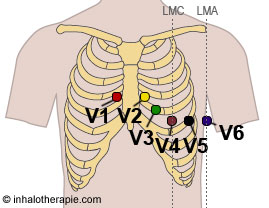
\includegraphics[scale=0.5]{derivations-precordiales.jpg}
  \source{Support de formation ECG}
\end{flashcard}


\color[HTML]{FF6D01}
\categ{PSE+}
\begin{flashcard}[bilan]{
 Décrire le sens de circulation du sang dans le coeur.   }
  \begin{itemize}
\item Le sang pauvre en oxygène entre dans l'oreillete droite
\item Le sang est chassé dans le ventricule droit.
\item La contraction ventriculaire chasse le sang vers l'artère pulmonaire pour qu'il se charge en oxygène.
\item Le sang oxygèné retourne dans le coeur via l'oreillete guache par les veines pulmonaires
\item le sang passe dans le ventricule gauche
\item La contraction ventriculaire chasse le sang riche vers les organes par l'aorte.
\end{itemize}
  \source{Support de formation ECG}
\end{flashcard}


\color[HTML]{FF6D01}
\categ{PSE+}
\begin{flashcard}[geste]{
 Dans quel cadre général (ambiance, etc.), doit-on réaliser un ECG ?   }
  Ambiance calme, température confortable, pas de contact avec un conducteur, éloignr les téléphones portables, éteindure le moteur d'un véhicule, favoriser l'adhésion des électrodes.
  \source{Support de formation ECG}
\end{flashcard}


\color[HTML]{FF6D01}
\categ{PSE+}
\begin{flashcard}[geste]{
 Comment installer une victime en vue de la réalisation d'un ECG ?   }
  Victime au repos allongée à plat dos, calme, bras et jambes décroisés, yeux fermés, sans parler, couverture. Informer du caractère sans risque et indolore.
  \source{Support de formation ECG}
\end{flashcard}


\color[HTML]{FF6D01}
\categ{PSE+}
\begin{flashcard}[geste]{
 Décrire le position des 4 électrodes périphériques.   }
  \begin{itemize}
 \item jaune sur poignet gauche
 \item vert sur cheville gauche
 \item noir sur cheville droiet 
\item rouge sur poignet droit
 \end{itemize}
Dans le sens des aiguilles d'une montre, Jeune Voyou Non Recommandable.
  \source{Support de formation ECG}
\end{flashcard}


\color[HTML]{FF6D01}
\categ{PSE+}
\begin{flashcard}[geste]{
 La victime a la main et l'avant-bras droit complètement brulés, comment placer les électrodes périphériques ?   }
  Poser alors les 4 électrodes à la racine des membres (épaules, hanches) et notifier à la coordination médicale cette pose.
  \source{Support de formation ECG}
\end{flashcard}


\color[HTML]{FF6D01}
\categ{PSE+}
\begin{flashcard}[geste]{
 La victime est en détresse respiratoire, comment réaliser l'ECG ?   }
  Il faut laisser la victime assise et notifier à la coordination médicale cette condition de réalisation de l'ECG. Les électrodes périphériques sont placés sur les épaules et sur les hances.
  \source{Support de formation ECG}
\end{flashcard}


\color[HTML]{FF6D01}
\categ{PSE+}
\begin{flashcard}[geste]{
 Quels sont les interférénces liées à la victime typiques lors de la réalisation d'un ECG ?   }
  \begin{itemize}
 \item tremblements dus au stress $\rightarrow$ rassurer (rapide, indolore, utile)
 \item tremblements dus au froid $\rightarrow$ couvrir
 \item tremblements pathologiques (type Parkinson) $\rightarrow$ poser à la racine des membres et notifier à la coordination médicale
 \end{itemize}
  \source{Support de formation ECG}
\end{flashcard}


\color[HTML]{FF6D01}
\categ{PSE+}
\begin{flashcard}[geste]{
 Quels sont les interférénces liées au matériel typiques lors de la réalisation d'un ECG ?   }
  \begin{itemize}
 \item lit médicalisé $\rightarrow$ débranché
 \item véhciule $\rightarrow$ éteindre le moteur, ne pas manipuler les portes, ne pas bouger
 \item mauvais contact des électrodes $\rightarrow$ raser/sécher, voire changer les électrodes
 \item téléphones portables $\rightarrow$ éloigner
 \end{itemize}
  \source{Support de formation ECG}
\end{flashcard}


\color[HTML]{FF6D01}
\categ{PSE+}
\begin{flashcard}[geste]{
 Quels signes sur le tracé d'un ECG peuvent indiquer une mauvaise pose des électrodes ?   }
  la présence d'une ligne plate sur au moins une dérivation
une ligne de base non-horizontale
  \source{Support de formation ECG}
\end{flashcard}


\color[HTML]{FF6D01}
\categ{PSE+}
\begin{flashcard}[geste]{
 Quel filtre peut-on ajouter pour nettoyer un ECG ?   }
  Dans lem enu ECG, selectionner "Filtres ECG", puis cocher "filtre EMG", en laissant coché "filtre BLW".
  \source{Support de formation ECG}
\end{flashcard}


\color[HTML]{01DFA5}
\categ{TECH}
\begin{flashcard}[radio]{
 Épeler en alphabet international "Usain Bolt" ?   }
  Uniform - Sierra - Alpha - India - November \\ Bravo - Oscar - Lima - Tango
  \source{Opérateur Radio FNPC.ppt}
\end{flashcard}


\color[HTML]{01DFA5}
\categ{TECH}
\begin{flashcard}[radio]{
 Compter de $0$ à $9$ en message radio   }
   zéro -- unité -- un et un -- deux et un -- deux et deux -- trois et deux -- trois fois deux -- quatre et trois -- deux fois quatre -- cinq et quatre
  \source{Opérateur Radio FNPC.ppt}
\end{flashcard}


\color[HTML]{01DFA5}
\categ{TECH}
\begin{flashcard}[radio]{
 Qu'est-ce qu'un indicatif ?   }
  C'est le nom de la station émettrice ou réceptrice.
  \source{Opérateur Radio FNPC.ppt}
\end{flashcard}


\color[HTML]{01DFA5}
\categ{TECH}
\begin{flashcard}[radio]{
 Concernant la radio, distinguer poste fixe, poste mobile et poste portatif.   }
  Un poste fixe est alimenté sur secteur et demeure sur un lieu. Un poste mobile est usuellement installé dans un véhicule (qui l'alimente). un poste portatif est un poste de taille réduite fonctionnant sur batteries.
  \source{Opérateur Radio FNPC.ppt}
\end{flashcard}


\color[HTML]{01DFA5}
\categ{TECH}
\begin{flashcard}[radio]{
 Expliciter les étapes de montage/démontage d'une radio. Quel est le point de vigilance fondamental ?   }
  Pour démonter, les étapes sont : éteindre, retirer la batterie, retirer l'antenne. \\ 
Pour remonter, les étapes sont : éteindre, placer l'antenne, placer la batterie. \\
Il ne faut jamais mettre allumer une radio sans son antenne, au risque de la détruire.
  \source{Opérateur Radio FNPC.ppt}
\end{flashcard}


\color[HTML]{01DFA5}
\categ{TECH}
\begin{flashcard}[radio]{
 Qu'est-ce qu'un réseau dirigé ? un réseau non-dirigé ?   }
  Un réseau dirigé a une station coordinatrice ("Poste de commandement"). Toutes les autres stations ne communiquent que vers et avec cette station coordinatrice, sauf sur son ordre. Exemple : régulation SAMU, DPS-GE, etc. \\
Sur un réseau non-dirigé, les stations peuvent communiquer entre elles. Exemple : PAPS, DPS-PE, etc.
  \source{Opérateur Radio FNPC.ppt}
\end{flashcard}


\color[HTML]{01DFA5}
\categ{TECH}
\begin{flashcard}[radio]{
 Sur un DPS, vous êtes la volante alpha et vous souhaitez signaler au poste de commandemant que vous prennez en charge une victime. Que dites-vous à la radio ?   }
  "Poste de commandement, poste de commandement, pour volante alpha" \\
"Volante alpha, transmettez." \\
"Prennons en charge une victime ... Terminé."
  \source{Opérateur Radio FNPC.ppt}
\end{flashcard}


\color[HTML]{01DFA5}
\categ{TECH}
\begin{flashcard}[radio]{
 Qui utilise le message clef "terminé" dans une conversation radio ?   }
  La station qui a initié la conversation.
  \source{Opérateur Radio FNPC.ppt}
\end{flashcard}


\color[HTML]{01DFA5}
\categ{TECH}
\begin{flashcard}[radio]{
 Comment accuser la réception d'une message transmis à tous ?   }
  "Reçu pour X" où X est mon indicatif radio.
  \source{Opérateur Radio FNPC.ppt}
\end{flashcard}


\color[HTML]{01DFA5}
\categ{TECH}
\begin{flashcard}[radio]{
 Que faire si votre interlocuteur vous demande de "collationnez" ?   }
  Il faut retransmettre le message que l'on vient de recevoir.
  \source{Opérateur Radio FNPC.ppt}
\end{flashcard}


\color[HTML]{01DFA5}
\categ{TECH}
\begin{flashcard}[radio]{
 Comment décrire la qualité du signal reçu ?   }
  Fort/faible pour le volume ; clair/haché pour la lisibilité.
  \source{Opérateur Radio FNPC.ppt}
\end{flashcard}


\color[HTML]{01DFA5}
\categ{TECH}
\begin{flashcard}[radio]{
 L'emploi de "affirmatif"/"négatif" est-il recommandé à la radio ?   }
  Non, car il peut y avoir des ambiguitiés en cas de phrase négative ("la patience ne présente pas d'équimose"). 
Préférez des phrase affirmatives ("aucun équimose n'est présent"), et l'emploi d'expression "C'est correct" ou "C'est incorrect". Pour demander confirmation, énoncer la phrase de manière affirmative et interroger "est-ce correct ?".
  \source{terrain}
\end{flashcard}


\color[HTML]{01DFA5}
\categ{TECH}
\begin{flashcard}[radio]{
 Quel message passé pour indiquer une erreur ?   }
  "Transmission annulée"
  \source{Opérateur Radio FNPC.ppt}
\end{flashcard}


\color[HTML]{01DFA5}
\categ{TECH}
\begin{flashcard}[radio]{
 Quel message passé pour vérifier que l'interlocuteur a recu le message ?   }
  "Accusez réception" ou "Est-ce reçu ? Parlez/transmettez."
  \source{Opérateur Radio FNPC.ppt}
\end{flashcard}


\color[HTML]{01DFA5}
\categ{TECH}
\begin{flashcard}[radio]{
 Quel message passé pour indiqué être informé d'un message sans en être destinataire ?   }
  "Interceptée pour X" où X est mon indicatif radio.
  \source{Opérateur Radio FNPC.ppt}
\end{flashcard}


\color[HTML]{01DFA5}
\categ{TECH}
\begin{flashcard}[radio]{
 Quelle est la procédure d'urgence ?   }
  En cas d'urgence, utiliser le schéma suivant : \\
"URGENT URGENT UREGENT PC de X, PC de X. Parlez" \\
"A tous de PC, silence radio. X parlez." \\
...
"A tous de PC, silence radio suspendu."

  \source{Opérateur Radio FNPC.ppt}
\end{flashcard}


\color[HTML]{01DFA5}
\categ{TECH}
\begin{flashcard}[véhicule]{
 Quel signe effectuer pour signifier "En arrière" au conducteur?   }
  Les deux bras fléchis, la paume des mains tournée vers le véhicule à hauteur des épaules, étendre les bras en direction du véhicule. \\     Exécuter ce mouvement plusieurs fois sil y a lieu.
  \source{DF-FICR-21 01 10 Guidage}
\end{flashcard}


\color[HTML]{01DFA5}
\categ{TECH}
\begin{flashcard}[véhicule]{
 Quel signe effectuer pour signifier "stop" au conducteur?   }
  Les deux bras en croix. \\ OU \\ Les deux bras tendus horizontalement dans lalignement des épaules
  \source{DF-FICR-21 01 10 Guidage}
\end{flashcard}


\color[HTML]{01DFA5}
\categ{TECH}
\begin{flashcard}[véhicule]{
 Quel signe effectuer pour signifier "attention" au conducteur?   }
  Bras droit levé verticalement, la paume de la main tournée vers lintérieur
  \source{DF-FICR-21 01 10 Guidage}
\end{flashcard}


\color[HTML]{01DFA5}
\categ{TECH}
\begin{flashcard}[véhicule]{
 Quel signe effectuer pour signifier "En avant" au conducteur?   }
  Les deux bras orientés vers le véhicule, la paume des mains tournée vers le visage, ramener les mains en direction des épaules.
Exécuter ce mouvement plusieurs fois sil y a lieu.
  \source{DF-FICR-21 01 10 Guidage}
\end{flashcard}


\color[HTML]{01DFA5}
\categ{TECH}
\begin{flashcard}[véhicule]{
 Quel signe effectuer pour signifier "En avant gauche" au conducteur?   }
  Le bras indiquant le sens du braquage est étendu dans la direction de braquage.
Exécuter le mouvement plusieurs fois sil y a lieu.
Lautre bras exécutant le mouvement « En avant ».
  \source{DF-FICR-21 01 10 Guidage}
\end{flashcard}


\color[HTML]{01DFA5}
\categ{TECH}
\begin{flashcard}[véhicule]{
 Quel signe effectuer pour signifier "En avant droite" au conducteur?   }
  Le bras indiquant le sens du braquage est étendu dans la direction de braquage.
Exécuter le mouvement plusieurs fois sil y a lieu.
Lautre bras exécutant le mouvement « En avant ».
  \source{DF-FICR-21 01 10 Guidage}
\end{flashcard}


\color[HTML]{01DFA5}
\categ{TECH}
\begin{flashcard}[véhicule]{
 Quel signe effectuer pour signifier "En arrière gauche" au conducteur?   }
  Le bras indiquant le sens du braquage est étendu dans la direction de braquage. Lautre bras exécutant le mouvement « En arrière ».
  \source{DF-FICR-21 01 10 Guidage}
\end{flashcard}


\color[HTML]{01DFA5}
\categ{TECH}
\begin{flashcard}[véhicule]{
 Quel signe effectuer pour signifier "En arrière droite" au conducteur?   }
  Le bras indiquant le sens du braquage est étendu dans la direction de braquage. Lautre bras exécutant le mouvement « En arrière ».
  \source{DF-FICR-21 01 10 Guidage}
\end{flashcard}


\color[HTML]{01DFA5}
\categ{TECH}
\begin{flashcard}[véhicule]{
 Qui est habilité à signifier aux secouristes qu'ils peuvent descendre du véhicule ?   }
  Le chauffeur uniquement.
  \source{A trouver ?}
\end{flashcard}


\color[HTML]{01DFA5}
\categ{TECH}
\begin{flashcard}[matériel]{
 Définir l'usage des lot A, lot B et lot C ?   }
  \begin{itemize}
        \item Le Lot A constitue le matériel minimum obligatoire pour équiper un poste de secours.
        \item Le Lot B constitue le matériel minimum obligatoire pour équiper un binôme sur poste de secours (mais un PAPS). Il ne doit pas être prélevé dans le VPS ou dans le lot A.
        \item Le lot C constitue le matériel minimum obligatoire pour équiper pour équiper une 2ème poste de secours ou un pour équiper un PAPS.
    \end{itemize}
  \source{FR DT-03-01 LOT VPS 2020}
\end{flashcard}


\color[HTML]{01DFA5}
\categ{TECH}
\begin{flashcard}[matériel]{
 Que contient un kit AES (Accident d'Exposition au Sang) ?   }
  \begin{tabular}{c|c}
        Désignation \& Quantité \\ \hline
        Paire de gants à usage unique \& 2 \\
        Compresses stériles \& 10 \\
        Flacon de Dakin 60 mL \& 2 \\
        Dispositif rince-oeil 500 mL \& 2 \\
        Flacon de prélèvement \& 1 \\
        Fiche-réflexe DF-28-01 \& 1
\end{tabular}
  \source{FR DF-29-02}
\end{flashcard}


\color[HTML]{01DFA5}
\categ{TECH}
\begin{flashcard}[matériel]{
 Que contient un kit Covid ?   }
  \begin{tabular}{c|c}
        Désignation \& Quantité \\ \hline
        Surblouse \& 2 \\
        Gants stériles \& 4 \\
        Masque FP2 \& 2 \\
        Paire de lunettes de protection \& 2 \\
        Charlotte \& 2 \\
        Sac DASRI \& 1 \\
        Glacon de gel hydroalcoolique \& 1 \\
        Masque chirugical \& 1
    \end{tabular}
  \source{à trouver}
\end{flashcard}


\color[HTML]{01DFA5}
\categ{TECH}
\begin{flashcard}[matériel]{
  Que contient un kit Accouchement ?   }
  \begin{tabular}{c|c}
        Désignation \& Quantité \\ \hline
        Clamp de Barr \& 3 \\
        compresses stériles \& 10 \\
        compresses non-tissés \& 1 paquet \\
        paire de gants stériles \& 1 \\
        champs stériles \& 2 \\
        pansement américain stérile \& 1 \\
        couverture de survie stérile \& 1 \\
        matériel aspiration pédia \& 1 \\
        dosettes de sérum physio \& 6 \\
        flacon de bétadine gynéco \& 1 \\
       bonnet + lunnette \& 1
    \end{tabular}
  \source{DOS-14-01 }
\end{flashcard}


\color[HTML]{01DFA5}
\categ{TECH}
\begin{flashcard}[matériel]{
 Que doit contenir une mallette DSA ?   }
  \begin{itemize}
        \item 1 DSA et sa carte mémoire
        \item Batterie ok (+1 de secours si possible)
        \item 2 patch adulte (non-périmés)
        \item 1 patch enfant (non périmé) -- si possible
        \item 2 rasoirs jetables
        \item 1 paquet de compresses -- si possible
        \item 1 paire de ciseaux Gesco
        \item administratif DSA PCPS
        \item adminsitratif DSA BSSP
    \end{itemize}
  \source{FR DOS-27-01}
\end{flashcard}


\color[HTML]{01DFA5}
\categ{TECH}
\begin{flashcard}[matériel]{
 Quel est le matériel d'immobilisation présent au sein d'un VPSP ?   }
  \begin{itemize}
        \item 5 colliers de différentes tailles
ou 1 collier réglable
        \item 3 attelles (jambe, avant bras, poignet)
        \item 2 écharpes + épingles-à-nourrice
        \item 1 MID avec drap + pompe
        \item 1 portoir souple       
        \item 1 brancard cuillère
        \item 1 brancard + 1 couverture bactériostatique + 1
drap
        \item 1 chaise à porteur
        \item 1 plan dur
        \item 3 sangles ou une sangle araignée
    \end{itemize}
  \source{FR DOS-28-01}
\end{flashcard}


\color[HTML]{01DFA5}
\categ{TECH}
\begin{flashcard}[matériel]{
 Quel est le matériel de bilan au sein d'un VPSP ?   }
  \begin{itemize}
        \item tensiomètre (4 brassards) + 1 stéthoscope
        \item thermomètre électronique
        \item oxymètre
        \item dextro (1 appareil, bandelettes, auto-piqueur)
    \end{itemize}
  \source{FR DOS-28-01}
\end{flashcard}


\color[HTML]{003273}
\categ{PSE}
\begin{flashcard}[bilan]{
 Comment évaluer l'impact psychologique d'une victime ?   }
  Les éléments révélant un potentiel impact psuchologique nécessite d'être recherchés et transmis au même titre que les paramètres vitaux.
\begin{itemize}
        \item présentation : visage, regard, comportement, gestuel, blessures)
        \item état de conscience : vigilance, mémoire, langage, jugement, raisonnement
        \item expression : conteu du dicours, émotions, état d'esprit, perception de l'environnements et des tiers
 \end{itemize}
  \source{Reco PSE 2021 - 01FT01}
\end{flashcard}


\color[HTML]{003273}
\categ{PSE}
\begin{flashcard}[geste]{
 Quels sont les principales actions pour stabiliser l'état psycho-physiologique d'une victime ?   }
  \begin{itemize}
        \item Demander à la victime de se focaliser sur le secouriste en utilisant duffrants canux de communication (voix, toucher, visuel)
        \item Déterminer un code de communication si besion (bruit important, impossibilité de parler, etc.)
        \item Suggérer un travail sur la respiration
        \item Encourager la victime à défocaliser son attention de la situation actuelle
        \item Expliquer et noramliser les réactions du corps
 \end{itemize}
  \source{Reco PSE 2021 - 01FT02}
\end{flashcard}


\color[HTML]{003273}
\categ{PSE}
\begin{flashcard}[geste]{
 Qu'est-ce que l'écoute active ? Quels sont les "4 R" de l'écoute active ?   }
  Lécoute active est une technique de communication qui consiste à utiliser le questionnement et la
reformulation afin de sassurer que lon a compris au mieux le message de son interlocuteur et de lui
démontrer. C'est une attitude ouverte et bienveillante.
\begin{itemize}
        \item Recontextualiser
        \item Reformuler
        \item Renforcer
        \item Résumer
 \end{itemize}
  \source{Reco PSE 2021 - 01FT03}
\end{flashcard}


\color[HTML]{003273}
\categ{PSE}
\begin{flashcard}[geste]{
 Qu'est-ce que la respiration contrôlée ? Quel est son usage dans le cadre du secourisme ?   }
  La relaction contrôlée est d'induire une respiration relaxante pour que la victime se détende et se calme. Elle peut aussi être utilisée par le souriste pour réguler son stress.
  \source{Reco PSE 2021 - 01FT04}
\end{flashcard}


\color[HTML]{003273}
\categ{PSE}
\begin{flashcard}[geste]{
 Dans le cadre d'une respiration contrôlée, décrire la \emph{respiration complète} ?   }
  La respiration complète consiste à mobliser (successivement ou simultanément) les trois étages respiratoires : abdomen, thorax, épaules.
Le temps d'expériation peut-être 3, 4 ou 5 fois supérieur au temps d'inspiration. 
Durée : 3 à 5 minutes.
  \source{Reco PSE 2021 - 01FT04}
\end{flashcard}


\color[HTML]{003273}
\categ{PSE}
\begin{flashcard}[geste]{
 Dans le cadre d'une respiration contrôlée, décrire la \emph{respiration abdominale} ?   }
  La respiration abdominale consiste gonler le ventre pour inspirer et à le rentrer pour expirer, sans mobiliser le thorax ni les épaules.
Le temps d'expériation peut-être 3, 4 ou 5 fois supérieur au temps d'inspiration. 
Durée : 3 à 5 minutes.
  \source{Reco PSE 2021 - 01FT04}
\end{flashcard}


\color[HTML]{003273}
\categ{PSE}
\begin{flashcard}[bilan]{
 Selon les recommandations de décembre 2021, quels sont les 4 bilans ?   }
  \begin{itemize} \item bilan circonstanciel (ou d'aproche) \item bilan d'urgence vitale \item bilan complémentaire \item bilans de surveilance \end{itemize}
  \source{Reco PSE 2021 - 02AC01}
\end{flashcard}


\color[HTML]{003273}
\categ{PSE}
\begin{flashcard}[bilan]{
 En quoi consiste globalement le bilan circontanciel ?   }
  Le bilan circonstanciel permet dapprécier la situation dans sa globalité, den évaluer les risques et de prendre les mesures adaptées notamment en ce qui concerne la sécurité.
  \source{Reco PSE 2021 - 02AC01}
\end{flashcard}


\color[HTML]{003273}
\categ{PSE}
\begin{flashcard}[bilan]{
 En quoi consiste globalement le bilan d'urgence vitale ?   }
  Le bilan durgence vitale qui a pour but de rechercher une détresse vitale qui menace immédiatement ou à très court terme la vie de la victime et nécessite la mise en uvre de gestes de secours immédiats.
  \source{Reco PSE 2021 - 02AC01}
\end{flashcard}


\color[HTML]{003273}
\categ{PSE}
\begin{flashcard}[bilan]{
 En quoi consiste globalement le bilan complémentaire ?   }
  Le bilan complémentaire qui permet de rechercher les autres signes dun malaise, dune maladie ou dun traumatisme, de les transmettre au médecin et de réaliser les gestes de premiers secours nécessaires.
  \source{Reco PSE 2021 - 02AC01}
\end{flashcard}


\color[HTML]{003273}
\categ{PSE}
\begin{flashcard}[bilan]{
 En quoi consiste globalement un bilan de surveillance ?   }
  La surveillance qui permet de suivre lévolution de létat de la victime, dévaluer lefficacité des gestes de secours effectués et denvisager, si nécessaire, une modification de sa prise en charge
  \source{Reco PSE 2021 - 02AC01}
\end{flashcard}


\color[HTML]{003273}
\categ{PSE}
\begin{flashcard}[geste]{
 Le retournement seffectue du côté opposé au visage de la victime.
Le secouriste 1, maitre de la manoeuvre,  en trépied, saisit ta tête  et accompangera le mvt (respecter tête-cou-tronc).
Le secouriste 2 se place sur le côté. Il étend le bras de la victime du côté du retournement et place la paume de l'autre main sous la cuisse de la victime. Il effectue le retournement en saisissant la victime à la hanche et à l'épaule. 
Le retournement s'effectue en deux temps avec une pause à 90° pour que le secouriste 2 pivote ses mains.   }
  Cette technique est indiquée après avoir constaté la perte de connaissance chez une victime sur le ventre.
Elle doit être réalisée systématiquement lorsque lon est en équipe et que la victime est suspecte dun traumastime du rachis.
Elle permet ensuite d'apprécier la respiration de la victime. réaliser les éventuels gestes d'urgence, puis de l'immobiliser pour un brancardage.
  \source{Reco PSE 2021 - 02FT01}
\end{flashcard}


\color[HTML]{003273}
\categ{PSE}
\begin{flashcard}[geste]{
 Décrire la mise en oeuvre d'un retournement à deux secouristes ?   }
  Le retournement seffectue du côté opposé au visage de la victime.
Le premier secouriste, maitre de la manoeuvre,  se place, en trépied, à la tête qu'il saisit et accompangera le mouvement pour respecter l'alignement tête-cou-tronc.
Le second secouriste se place sur le côté de la vitcime. Il étend le bras de la victime du côté du retournement ("superman") et place la paume de l'autre main sous la cuisse de la victime. Il effectue le retournement en saisissant la victime à la hanche et à l'épaule. 
Le retournement s'effectue en deux temps avec une pause courte à 90° pour que le secouriste 2 puisse repositionner ses mains.
Laxe tête-cou-tronc de la victime doit être maintenu le plus rectiligne possible tout au long du retournement
  \source{Reco PSE 2021 - 02FT01}
\end{flashcard}


\color[HTML]{003273}
\categ{PSE}
\begin{flashcard}[geste]{
 Donner une séquence générale d'ordre pour une manoeuvre et la distinction entre un ordre préparatoire et un ordre exécutoire.   }
  Le secouriste à la tête de la victime est le coordinateur qui donne les ordres. La séquence générale est la suivante :
"-Secouristes des pieds à la tête, êtes-vous prêts ?
- Pieds, pret.
...
- Secouristes, pret pour tourner. Tournez."
"Prêt pour tourner" est un ordre préparatoire qui annonce l'imminence de l'action. "Tournez" est l'ordre exécutoire, qui est toujours précédé d'un ordre préparatoire.
  \source{}
\end{flashcard}


\color[HTML]{003273}
\categ{PSE}
\begin{flashcard}[geste]{
 Quand réalise-t-on un retournement à un secouriste ?   }
  Cette technique est indiquée après avoir constaté la perte de connaissance chez une victime sur le ventre lorsque le secouriste est seul. Elle permet ensuite d'apprécier la respiration de la victime et de réaliser les éventuels gestes d'urgence.
  \source{Reco PSE 2021 - 02FT02}
\end{flashcard}


\color[HTML]{003273}
\categ{PSE}
\begin{flashcard}[geste]{
 Décrire la mise en oeuvre d'un retournement à un  secouriste ?   }
  Le retournement seffectue du côté opposé au visage de la victime : 
\begin{itemize}
\item placer le bras de la victime du côté du retournement au-dessus de sa tête
\item du côté du retournement saisir par lépaule et la hanche 
\item faire rouler doucement et dun bloc la victime à 90°
\item glisser la main qui était à lépaule au niveau de la nuque de la victime (avant-bras contre le dos)
\item tirer sur la hanche
\end{itemize}
  \source{Reco PSE 2021 - 02FT02}
\end{flashcard}


\color[HTML]{003273}
\categ{PSE}
\begin{flashcard}[geste]{
 Chez une victime de malaise ou malade, quels sont les éléments à rechercher.   }
  \begin{itemize}
\item asymétrie de l'expression faciale
\item faiblesse musculaire d'un membre supérieur
\item anomalie de la parole
\item mesure de glycémie
\item mesure de la température
\end{itemize}

  \source{Reco PSE 2021 - 02FT03}
\end{flashcard}


\color[HTML]{003273}
\categ{PSE}
\begin{flashcard}[geste]{
 Chez une victime d'un traumatisme, comment qualifier la ou les lésion(s).   }
  Pour chaque lésion, il faut préciser sa nature (contusions, gonflement, déformations, plaies, brulures, etc.), sa localition exacte et son étendue.
  \source{Reco PSE 2021 - 02FT03}
\end{flashcard}


\color[HTML]{003273}
\categ{PSE}
\begin{flashcard}[geste]{
 Comment effectuer la recherche de lésion chez une victime d'un traumatisme.   }
  Il faut effectuer la recherche sur le corps entier, de la tête au pied, en examinant ou en plapant (sauf le bassin).
  \source{Reco PSE 2021 - 02FT03}
\end{flashcard}


\color[HTML]{003273}
\categ{PSE}
\begin{flashcard}[geste]{
 Chez une victime d'un traumatisme, comment effectuer l'examen de la tête ?   }
  Passer les mains dans les cheveux et observer la face à la recherche dun saignement ou dune déformation (hématome autour des yeux, etc.). Repérer un écoulement par le nez ou les oreilles.
  \source{Reco PSE 2021 - 02FT03}
\end{flashcard}


\color[HTML]{003273}
\categ{PSE}
\begin{flashcard}[geste]{
 Chez une victime d'un traumatisme, comment effectuer l'examen du cou?   }
  Après avoir stabilisé le rachis cervical, observer et passer les mains sous la nuque sans déplacer ni surélever la tête à la recherche de sang, dune douleur ou dune déformation
  \source{Reco PSE 2021 - 02FT03}
\end{flashcard}


\color[HTML]{003273}
\categ{PSE}
\begin{flashcard}[geste]{
 Chez une victime d'un traumatisme, comment effectuer l'examen du thorax ?   }
  Rechercher une contusion, une plaie et une anomalie du soulèvement de la poitrine à la respiration (seule une partie du thorax se soulève).
  \source{Reco PSE 2021 - 02FT03}
\end{flashcard}


\color[HTML]{003273}
\categ{PSE}
\begin{flashcard}[geste]{
 Chez une victime d'un traumatisme, comment effectuer l'examen de l'abdomen ?   }
  Rechercher une contusion ou une plaie de labdomen (parfois accompagnée dune sortie de lintestin). Apprécier le soulèvement de labdomen à chaque inspiration. Appuyer délicatement sur la paroi de labdomen à la recherche dune douleur provoquée.
  \source{Reco PSE 2021 - 02FT03}
\end{flashcard}


\color[HTML]{003273}
\categ{PSE}
\begin{flashcard}[geste]{
 Chez une victime d'un traumatisme, comment effectuer l'examen du dos ?   }
  Glisser les mains sous la victime sans la mobiliser et sans la déplacer à la recherche dun saignement ou dune douleur. Le secouriste peut profiter dune manoeuvre de relevage ou du déplacement de la victime pour faire cette recherche.
  \source{Reco PSE 2021 - 02FT03}
\end{flashcard}


\color[HTML]{003273}
\categ{PSE}
\begin{flashcard}[geste]{
 Chez une victime d'un traumatisme, comment effectuer l'examen deu bassin ?   }
  Aucune palpation du bassin ne doit être réalisée. Un traumatisme du bassin est suspecté devant une
victime qui se plaint dune douleur spontanée de la partie basse de labdomen ou du bassin. Noter la
présence de taches de sang sur les sous-vêtements qui peut faire suspecter un traumatisme des
organes génitaux ou urinaires.
Si la victime a perdu connaissance, une fracture du bassin sera suspectée chez toutes les victimes
traumatisées qui présentent des signes de détresse circulatoire.
  \source{Reco PSE 2021 - 02FT03}
\end{flashcard}


\color[HTML]{003273}
\categ{PSE}
\begin{flashcard}[geste]{
 Chez une victime d'un traumatisme, comment effectuer l'examen des membres  ?   }
  L'examen est à mener sur les 4 membres, si possible sans chaussures ni chaussette. \\
\begin{itemize}
\item Rechercher l'état de la circulation à l'extrémité (coloration, température, TRC, pouls)
\item Tester la motricité 
\item Teste la sensibilité
\end{itemize}
La palpation s'effectue à deux mains avec empaument latéral délicat de la racine à l'extrémité du membre.
  \source{Reco PSE 2021 - 02FT03}
\end{flashcard}


\color[HTML]{003273}
\categ{PSE}
\begin{flashcard}[geste]{
 Dans quels cas une mesure de la glycémie est à envisager.   }
  \begin{itemize} \item signes d'un AVC \item malaise suceptible d'être liée à une hypoglycémie (diabétique, effort à jeun) \item trouble du comportement \item perte de connaisance \end{itemize}
  \source{Reco PSE 2021 - 02FT05}
\end{flashcard}


\color[HTML]{003273}
\categ{PSE}
\begin{flashcard}[bilan]{
 En cas de nombreuses victimes, quel est le code couleur de repérage ?   }
  \begin{itemize} \item Noir : victime décédée, victime inconsciente qui ne respire pas après une LVA \item Rouge : victime inconsciente qui respire (après LVA), détrelle vitale évidente (FR ou FC), victime d'une hémoragie \item Jaune : victime consciente sans détresse vitale et immobile \item Vert : victime consciente sans détresse vitale qui peut se dépalcer \end{itemize}
  \source{Reco PSE 2021 - 02FT10}
\end{flashcard}


\color[HTML]{003273}
\categ{PSE}
\begin{flashcard}[matériel]{
 Donner l'ordre des actions pour se vêtir d'un équipement de protection complet (lutte contre le covid par exemple).   }
  \begin{enumerate} \item Se laver les mains \item mettre la charlotte \item mettre la surblouse \item mettre le masque \item mettre les lunettes de protection \item mettre les gants \end{enumerate}
  \source{Reco PSE 2021 - 04FT01}
\end{flashcard}


\color[HTML]{003273}
\categ{PSE}
\begin{flashcard}[matériel]{
 Donner l'ordre des actions pour se dévêtir d'un équipement de protection complet (lutte contre le covid par exemple).   }
  \begin{enumerate} \item retirer les lunettes \item retirer le masque \item retirer la charlotte \item retirer la sur-blouse en la retournant \item retirer les gants en les retournants \end{enumerate} 
Les équipments souillés doivent être jetés dans un DASRI.
  \source{Reco PSE 2021 - 04FT01}
\end{flashcard}


\color[HTML]{003273}
\categ{PSE}
\begin{flashcard}[matériel]{
 Quels sont les niveau de protocole de nettoyage d'un véhicule ou d'un local ? Les décrire succintement.   }
  \begin{itemize} \item le protocole simplifié : entre chauqe prise en charge \item protocole de début de mission : à chaque nouvelle mission \item protocole appronfondie : à l'issue de la prise en charge d'une victime à risque infectieux ou de manière périodique \end{itemize}
 L'entretien assure la propreté visuelle et la propreté microbiologique.
  \source{Reco PSE 2021 - 04FT05}
\end{flashcard}


\color[HTML]{003273}
\categ{PSE}
\begin{flashcard}[matériel]{
 Comment procéder au protocole simplifée de nettoyage d'un véhicule ou d'un local (P1) ?   }
  Le nettoyage s'effctue avec des gants de protection, dans un espace aérée si possible après s'être lavé les mains. \\ \begin{itemize} \item pulvériser une solution détergente-désinfectante sur le matériel exposé \item étaler la solution à l'aide d'une lavette \item laisser sécher et ne pas rincer \item jetter la lavette dans un DSARI \end{itemize}
  \source{Reco PSE 2021 - 04FT05}
\end{flashcard}


\color[HTML]{003273}
\categ{PSE}
\begin{flashcard}[matériel]{
 Comment procéder au protocole de nettoyage de début de mission d'un véhicule ou d'un local (P2) ?   }
  Le nettoyage s'effctue avec des gants de protection, dans un espace aérée si possible après s'être lavé les mains. \\ \begin{itemize} \item nettoyer et désinfecter la cellue sanitaire en otant le matériel encombrant, nettoyant les surfaces du sol au plafond et de l'intérieur vers l'extérieur avec la technique des "2 seauxs" (changer les seaux pour le sol) \item nettoyager et désinfecter la cabine de conduite selon la même méthode \end{itemize}
  \source{Reco PSE 2021 - 04FT05}
\end{flashcard}


\color[HTML]{003273}
\categ{PSE}
\begin{flashcard}[matériel]{
 Comment procéder au protocole de nettoyage appronfondi d'un véhicule ou d'un local (P3) ?   }
  Le nettoyage s'effctue avec des gants de protection, dans un espace aérée si possible après s'être lavé les mains. \\ \begin{itemize} \item nettoyer et désinfecter la cellue sanitaire en otant le matériel encombrant, nettoyant les surfaces du sol au plafond et de l'intérieur vers l'extérieur avec la technique des "2 seaus" (changer les seaux pour le sol), yc tirroirs et placards. \item nettoyer et désinfecter la cabine \item nettoyer et désinfecter le matériel, vérifier son fonctionnement avant réintégration \end{itemize}
  \source{Reco PSE 2021 - 04FT05}
\end{flashcard}


\color[HTML]{003273}
\categ{PSE}
\begin{flashcard}[matériel]{
 Décrire la technique dite des "2 seaux". Dans quels cas s'utilise-t-elles ?   }
  La technique de "2 seaux" s'utilise pour la P2 et la P3. \\ \begin{itemize} \item Remplir le seau rouge avec une solution lavante et le seau bleu avec de l'eau propre \item tremper la frange dans le seau rouge \item nettoyer le sol du fond vers l'extérieur en faisant des "S" \item essorer la frange dans le seau bleu \item tremper la frange dans le seau rouge \end{itemize}
  \source{Reco PSE 2021 - 05AC01}
\end{flashcard}


\color[HTML]{003273}
\categ{PSE}
\begin{flashcard}[matériel]{
 Quel est la différence entre un agent détergent et un agent désinfectant ?   }
  Un détergent est un produit nettoyant qui rend propre visuellement : il retire les tâches mais n'a pas d'action antimicrobienne. Il est ensio-actif. \\ Un désinfectant est un produit qui ne peut être utilisé que sur des surface propre pour éliminer, inactiver ou tuer les microorganismes (bactéries, virus, etc.) après un temps détersion. C'est pour cela qu'il faut laisser sécher et non rincer le matériel lors des protocoles de nettoyage.
  \source{Reco PSE 2021 - 04FT08}
\end{flashcard}


\color[HTML]{003273}
\categ{PSE}
\begin{flashcard}[bilan]{
 Qu'est-ce qu'un arrêt cardiaque ? Quelles sont les causes usuelles chez l'adulte ?   }
  Une personne est en arrêt cardiaque (AC) lorsque son coeur ne fonctionne plus ou fonctionne de façon anarchique. \\
Chez l'adulte, l'arrêt cardiaque : \begin{itemize} \item est le plus souvent d'origne cardiaque \item peut avoir une origine respiratoire (OVA, trauma crânien/rachis/thorax, noyade, pendaison, électrification) \item ou survenir à la suite d'une hémorragie \end{itemize}
  \source{Reco PSE 2021 - 05AC01}
\end{flashcard}


\color[HTML]{003273}
\categ{PSE}
\begin{flashcard}[bilan]{
 Qu'est-ce qu'un arrêt cardiaque ? Quelles sont les causes usuelles chez un enfant ou un nourrisson ?   }
  Une personne est en arrêt cardiaque (AC) lorsque son coeur ne fonctionne plus ou fonctionne de façon anarchique. \\
Chez l'enfant ou le nourrison , l'arrêt cardiaque : \begin{itemize} \item est le plus souvent à cause d'une maladie cardiaque non connue \item peut être d'origne respiratoire (étouffement, strangulation, OVA, noyade) \item plus rarement faire suite à une méorragie, une électrification ou un traumatisme (crâne/rachis/thorax). \end{itemize}
  \source{Reco PSE 2021 - 05AC01}
\end{flashcard}


\color[HTML]{003273}
\categ{PSE}
\begin{flashcard}[bilan]{
 Quels sont les signes guidant la CAT d'un arrêt cardiaque ? (et non les signes cliniques de l'imminence d'un AC).   }
  L'identification s'effectue en qq secondes lors du bilan d'urgence vitale. \\ Une victime est considérée en AC si elle ne répond pas (inconscience) et ne reprise plus (ou présente une respiration agonique).
  \source{Reco PSE 2021 - 05AC01}
\end{flashcard}


\color[HTML]{003273}
\categ{PSE}
\begin{flashcard}[bilan]{
 Décrire la conduite à tenir pour une victime    }
  \begin{tabular}{ccccc}
         Prise   \& Cons- \& Venti- \& Pouls \& CAT \\ 
         de poul \&     -cience       \& -lation       \&       \& \\ \hline
         non \& non \& oui \& X \& PLS \\
         non \& non \& non\& X \& RCP\\
         oui \& oui \& oui \& bien perçu \& PLS \\
         oui \& non \& non \& non \& RCP \\
         oui \& oui \& non \& non \& RCP \\
         oui \& non \& non \& oui \& Insuflation
\end{tabular}
  \source{Reco PSE 2021 - 05AC01}
\end{flashcard}


\color[HTML]{003273}
\categ{PSE}
\begin{flashcard}[bilan]{
 Au bout de combien de temps un arrêt cardiaque est fatal ? Quel gain représente la pause précoce d'un DAE ?   }
  Les lésions provoquées par un arrêt cardiaque deviennent progressivement irréversibles avec des chances de survie quasi-nulle au bout de 8 minutes environ. La chaine de secours est suceptible d'augementer de 4 à 40 \% le taux de survie des victimes. Chaque minute gagnée pour la pose d'un DAE peut augmenter de 10 \% les chances de survie.
  \source{Reco PSE 2021 - 05AC01}
\end{flashcard}


\color[HTML]{003273}
\categ{PSE}
\begin{flashcard}[bilan]{
 Quels sont les signes anonciateur d'un arrêt cardiaque ?   }
  Les signes annonciateurs sont : douleur serrant la poitrine, permanante, angoisante pouvant irradier dans le cou et les bras. La douleur est parfois associée à une difficulté à repsirer et à des sueurs.
  \source{Reco PSE 2021 - 05AC01}
\end{flashcard}


\color[HTML]{003273}
\categ{PSE}
\begin{flashcard}[bilan]{
 Chez la femme, quels sont les signes supplémentaires les plus courants d'un arrêt cardiaque ?   }
  Chez la femme, les signes anonciateurs spécifiques d'un arret cardiaque par infarctus du myocarde sont : \begin{itemize} \item étourdissement soudain \item sensation de brûlures d'estomac \item naussés ou vomissements \item sueurs froides \item fatigues inhabituelles \end{itemize}
  \source{Fondation "Agir pour le coeur des femmes"}
\end{flashcard}


\color[HTML]{003273}
\categ{PSE}
\begin{flashcard}[CAT]{
 Décrire la RCP chez l'adulte à 2 secouristes sans DAE (type volante du pauvre de DPS).   }
  \begin{itemize} \item Débuter immédiatement la RCP en cycle de 30-2, à un rythme de 120 compressions par minute \item Un secouriste effetue la RCP tandis que l'autre  demande de renfort médical puis va chercher un DAE pour pose asap \item Suivre les consignes du DAE \item Sans retarder la RCP, si possible adminitrer de l'$O_2$ \item Sans retarder la RCP, si nécessaire, aspirer les sécrétions \item Mettre en place une canule oropharyngée si nécessaire. \end{itemize} 
  \source{Reco PSE 2021 - 05PR01}
\end{flashcard}


\color[HTML]{003273}
\categ{PSE}
\begin{flashcard}[CAT]{
 Décrire la RCP chez l'adulte à 2 secouristes avec DAE (type volante de DPS).   }
  \begin{itemize} \item Débuter immédiatement la RCP en cycle de 30-2, à un rythme de 120 compressions par minute \item Un secouriste effetue la RCAP tandis que l'autre pose le DAE. \item La demande de renfort médical immaditement après la première analyse \item Suivre les consignes du DAE \item Sans retarder la RCP, si possible adminitrer de l'$O_2$ \item Sans retarder la RCP, si nécessaire, aspirer les sécrétions \item Mettre en place une canule oropharyngée si nécessaire. \end{itemize}
  \source{Reco PSE 2021 - 05PR01}
\end{flashcard}


\color[HTML]{003273}
\categ{PSE}
\begin{flashcard}[CAT]{
 Décrire la RCP chez l'adulte à 3 secouristes ou plus avec ou sans DAE.   }
  \begin{itemize} \item Débuter immédiatement la RCP en cycle de 30-2, à un rythme de 120 compressions pa rminute \item Un secouriste effetue la RCAP, un second pose le DAE, le troisième passer l'alerte. \item Suivre les consignes du DAE \item Sans retarder la RCP, si possible adminitrer de l'$O_2$ \item Sans retarder la RCP, si nécessaire, aspirer les sécrétions \item Mettre en place une canule oropharyngée si nécessaire. \end{itemize} Se relayer toutes les deux minutes.
  \source{Reco PSE 2021 - 05PR01}
\end{flashcard}


\color[HTML]{003273}
\categ{PSE}
\begin{flashcard}[CAT]{
 Décrire la RCP chez l'adulte avec un secouriste isolé sans tiers.   }
  \begin{itemize} \item Passer l'alerte \item Si un DAE est à proximité immédiate, le mettre en place le plus tôt possible, et suivre les consignes du DAE \item Sinon, débuter immédiatement la RCP en cycle de 30-2, à un rythme de 120 compressions par minute  \end{itemize} 
  \source{Reco PSE 2021 - 05PR02}
\end{flashcard}


\color[HTML]{003273}
\categ{PSE}
\begin{flashcard}[CAT]{
 Décrire la RCP chez l'adulte avec un secouriste isolé avec un tiers.   }
  \begin{itemize} \item Faire alerter par le tiers \item Si un DAE est à proximité immédiate, le mettre en place ou le faire mettre en place le plus tôt possible, et suivre les consignes du DAE \item Sinon, débuter immédiatement la RCP en cycle de 30-2, à un rythme de 120 compressions par minute  \end{itemize} 
  \source{Reco PSE 2021 - 05PR02}
\end{flashcard}


\color[HTML]{003273}
\categ{PSE}
\begin{flashcard}[CAT]{
 Décrire la RCP chez l'enfant ou le nourrison à 2 secouristes sans DAE (type volante du pauvre de DPS).   }
  \begin{itemize} \item retirer tout corps étranger visible de la bouche \item réaliser 5 insuflations starter \item passer l'alerte médicale \item Débuter immédiatement la RCP en cycle de 15-2, à un rythme de ??? compressions par minute \item Sans retarder la RCP, si possible adminitrer de l'$O_2$ \item Sans retarder la RCP, si nécessaire, aspirer les sécrétions \item Mettre en place une canule oropharyngée si nécessaire. \end{itemize}
  \source{Reco PSE 2021 - 05PR03}
\end{flashcard}


\color[HTML]{003273}
\categ{PSE}
\begin{flashcard}[CAT]{
 Lors d'une RCP à plusieures secouristes, à quelle fréquence se relayer idéalement ?   }
  Se relayer toutes les deux minutes
  \source{Reco PSE 2021 - 05PR03}
\end{flashcard}


\color[HTML]{003273}
\categ{PSE}
\begin{flashcard}[CAT]{
 Décrire la RCP chez l'enfant ou le nourrisson à 2 secouristes avec DAE (type volante de DPS).   }
  \begin{itemize} 
\item retirer tout corps étranger visible de la bouche 
\item réaliser 5 insuflations starter 
\item passer l'alerte médicale 
\item Débuter immédiatement la RCP en cycle de 15-2, à un rythme de ??? compressions par minute, tandis que l'autre secouriste pose le DAE 
\item Sans retarder la RCP, si possible adminitrer de l'$O_2$ et si nécessaire, aspirer les sécrétions et/ou mettre en place une canule oropharyngée\end{itemize} 
  \source{Reco PSE 2021 - 05PR03}
\end{flashcard}


\color[HTML]{003273}
\categ{PSE}
\begin{flashcard}[CAT]{
 Décrire la RCP chez l'enfant à 3 secouristes ou plus avec ou sans DAE.   }
  \begin{itemize} 
\item retirer tout corps étranger visible de la bouche 
\item réaliser 5 insuflations starter 
\item passer l'alerte médicale 
\item Débuter immédiatement la RCP en cycle de 15-2, à un rythme de \color{red}{???} compressions par minute, tandis que l'autre secouriste pose le DAE 
\item Sans retarder la RCP, si possible adminitrer de l'$O_2$ et si nécessaire, aspirer les sécrétions et/ou mettre en place une canule oropharyngée
 \end{itemize} 
  \source{Reco PSE 2021 - 05PR03}
\end{flashcard}


\color[HTML]{003273}
\categ{PSE}
\begin{flashcard}[CAT]{
 Décrire la RCP chez l'enfant avec un secouriste isolé sans tiers.   }
  \begin{itemize} 
\item retirer tout corps étranger visible de la bouche 
\item réaliser 5 insuflations starter 
\item passer l'alerte médicale 
\item Débuter immédiatement la RCP en cycle de 15-2, à un rythme de \color{red}{???} compressions par minute 
\item Si un DAE est à proximité immédiate, le mettre en place le plus tôt possible, et suivre les consignes du DAE , ou reprendre la RCP \end{itemize} 
  \source{Reco PSE 2021 - 05PR04}
\end{flashcard}


\color[HTML]{003273}
\categ{PSE}
\begin{flashcard}[CAT]{
 Décrire la RCP chez l'enfant avec un secouriste isolé avec un tiers.   }
  \begin{itemize} 
\item faire alerter et récalmer un DAE 
\item retirer tout corps étranger visible de la bouche 
\item réaliser 5 insuflations starter 
\item passer l'alerte médicale 
\item Débuter immédiatement la RCP en cycle de 15-2, à un rythme de \color{red}{???} compressions par minute 
\item poser ou faire poser dès que possible le DAE 
\end{itemize} 
  \source{Reco PSE 2021 - 05PR04}
\end{flashcard}


\color[HTML]{003273}
\categ{PSE}
\begin{flashcard}[bilan]{
 Qu'est-ce qu'une détresse circulatoire?   }
  On appelle détresse circulatoire une atteinte de la fonction circulatoire dont lévolution peut affecter, à court terme, les autres fonctions vitales de lorganisme (fonction respiratoire, fonction neurologique) et conduire au décès de la victime. \\ L'arrête cardiaque est une détresse circulatoire majeure, mais il en existe d'autres.
  \source{Reco PSE 2021 - 05AC02}
\end{flashcard}


\color[HTML]{003273}
\categ{PSE}
\begin{flashcard}[bilan]{
 Quels sont les principales causes d'une détresse circulatoire?   }
  \begin{itemize} \item atteinte du coeur (infarctus, insuffisance cardique) \item diminution de la quantité de sang (hémorragie, déshydratation) \item dilataion des vaissaux sanguins (réaction allergiques, intoxications graves \end{itemize}
  \source{Reco PSE 2021 - 05AC02}
\end{flashcard}


\color[HTML]{003273}
\categ{PSE}
\begin{flashcard}[bilan]{
 Quels sont les principaux signes d'une détresse circulatoire?   }
  \begin{itemize} \item insconcience sans respiration \item poul non perçu \item PA systolique $< 90$mmHg (ou baisse de 30\% si hypertendu) \item $FC>120$ ou $FC<40$ \item $TRC > 3$sec \item pâleur des extrémités, conjonctive, lèvres \item marbures cutanées ($++$ genoux), \item sueurs froides \item soif \item agittion, angoisse de mort \item vertiges, somnolence, perte ce connaissance \end{itemize}
  \source{Reco PSE 2021 - 05AC02}
\end{flashcard}


\color[HTML]{003273}
\categ{PSE}
\begin{flashcard}[CAT]{
 Quel est le principe d'action en cas de détresse circulatoire ?   }
  \begin{itemize} \item arreter uneéventuelle hémorragie externe \item améliorerl'oxygénation \item demander une aide médicale \item surveillance renforcée \end{itemize}
  \source{Reco PSE 2021 - 05AC02}
\end{flashcard}


\color[HTML]{003273}
\categ{PSE}
\begin{flashcard}[CAT]{
 Quel est la CAT pour une victime conscience en cas de detresse circulatoire non-hémmoragique (ou après avoir arrêté une hémorragie) ?   }
  \begin{itemize} \item allonger la victime \item administrer de l'oxygène par inhalation \item protéger du froid \item compléter le bilan d'urgce vitale, et réaliser un bilan complémentaire \item demander un avis médical \item surveiller la victime \end{itemize} Le risque d'aggravtion brutale avec AC est majeur,notament en cas de relevage ou de brancardage.
  \source{Reco PSE 2021 - 05PR05}
\end{flashcard}


\color[HTML]{003273}
\categ{PSE}
\begin{flashcard}[bilan]{
 Qu'est-ce qu'une détresse neurologique?   }
  On appelle détresse neurologique une atteinte de la fonction nerveuse dont lévolution peut affecter, à court terme, les autres fonctions vitales de lorganisme (fonction circulatoire, fonction respiratoire) et conduire au décès de la victime. \\ 
La perte de connaissance est une détresse majeure mais il en existe d'autres.
  \source{Reco PSE 2021 - 05AC03}
\end{flashcard}


\color[HTML]{003273}
\categ{PSE}
\begin{flashcard}[bilan]{
 Quelles sont les principales causes d'une détresse neurologique ?   }
  \begin{itemize} \item traumatisme, notamment cranien \item maladie atteignant le cerveu, la moelle épinière ou les nerfs \item intoxications \item manque de sucre \end{itemize}
  \source{Reco PSE 2021 - 05AC03}
\end{flashcard}


\color[HTML]{003273}
\categ{PSE}
\begin{flashcard}[bilan]{
 Quels sont les principaux signes d'une détresse neurologique ?   }
  \begin{itemize} \item perte de connaissance \item altération de la conscience \item convulsion \item désorientation \item amnésie \item paralysie \item asymétrie du visage \item asymétrie des pupilles \item aréactivité des pupilles \item anomalie de la parole \end{itemize}
  \source{Reco PSE 2021 - 05AC03}
\end{flashcard}


\color[HTML]{003273}
\categ{PSE}
\begin{flashcard}[CAT]{
 Quel est le principe d'action en cas de détresse neurologique ?   }
  \begin{itemize} \item installer la victime dans une position adaptée afin de préserver la circulation cérébrale \item obtenir une aide médicale \item surveillance renforcée \end{itemize}
  \source{Reco PSE 2021 - 05AC03}
\end{flashcard}


\color[HTML]{003273}
\categ{PSE}
\begin{flashcard}[CAT]{
 Quel est la CAT pour victime de détresse neurologique ?   }
  Dans le cas d'une victime consciente, \begin{itemize} \item allonger la victime avec protection contre le froid \item administrer de l'oxygène si nécessaire \item compléter le bilan d'urgence vitale \item réaliser le bilan complémentaire, et prodiguer les gestes de secours nécessaires \item demander un avis médical \item surveillance renforcée \end{itemize}
  \source{Reco PSE 2021 - 05PR06}
\end{flashcard}


\color[HTML]{003273}
\categ{PSE}
\begin{flashcard}[bilan]{
 Qu'est-ce qu'une détresse respiratoire ?   }
  On appelle détresse respiratoire une atteinte de la fonction respiratoire dont lévolution peut affecter, à court terme, les autres fonctions vitales de lorganisme (fonction circulatoire, fonction neurologique) et conduire au décès de la victime. \\ L'arrêt respiratoire est une détresse majeure mais il en existe d'autres.
  \source{Reco PSE 2021 - 05AC04}
\end{flashcard}


\color[HTML]{003273}
\categ{PSE}
\begin{flashcard}[bilan]{
 Quelles sont les principales causes d'une détresse respiratoire ?   }
  \begin{itemize} \item obstruction complète ou partielle des voies aériennes (corps étranger, allergie, traumatisme ou infection),
\item les maladies pulmonaires dont lasthme
\item le traumatisme du thorax 
\item linhalation de produits caustiques ou de fumées \end{itemize}
  \source{Reco PSE 2021 - 05AC04}
\end{flashcard}


\color[HTML]{003273}
\categ{PSE}
\begin{flashcard}[bilan]{
 Quels sont les principaux signes d'une détresse respiratoire ?   }
  \begin{itemize}
 \item plainte de la victime : gêne, respiraiton, effouffement, veut rester assis, etc.
\item respiration : FR $>30$ MPM, superficielle ou bruyante 
\item $SpO_2<94\%$ (ou $<89\%$ pour IRC) 
\item sueurs, cyanose 
\item confusion, somnolence, anxigeuse, agitation 
\item battement des ailes du nez et signe de tirage
 \item difficulté à parler
\end{itemize}
  \source{Reco PSE 2021 - 05AC04}
\end{flashcard}


\color[HTML]{003273}
\categ{PSE}
\begin{flashcard}[bilan]{
 Quel est le principe d'action en cas de détresse respiratoire ?   }
  \begin{itemize} \item arrêter immédiatement toute cause évidense (type OVA) \item améliorer l'oxygénation \item obtenir de l'aide médicale \item surveillance renforcée \end{itemize}
  \source{Reco PSE 2021 - 05AC04}
\end{flashcard}


\color[HTML]{003273}
\categ{PSE}
\begin{flashcard}[CAT]{
 Quel est la CAT pour victime de détresse respiratoire?   }
  Dans le cas d'une victime consciente, \begin{itemize} 
\item ne jamais allonger la victime ; préférer la position la plus confortable (assise ou demi-assise)
\item desserrer tous les vêtements pouvant gênant la respiration
\item administrer de l'oxygène si nécessaire 
\item compléter le bilan d'urgence vitale 
\item réaliser le bilan complémentaire, et prodiguer les gestes de secours nécessaires 
\item demander un avis médical 
\item surveillance renforcée \end{itemize}
  \source{Reco PSE 2021 - 05PR07}
\end{flashcard}


\color[HTML]{003273}
\categ{PSE}
\begin{flashcard}[bilan]{
 Qu'est ce qu'une hémorragie externe et quelles en sont les causes ?   }
  Une hémorragie externe est un épanchement de sang abondant et visible, qui sécoule en dehors des vaisseaux au travers dune plaie et ne sarrête pas spontanément. \\ 
Lhémorragie externe est le plus souvent dorigine traumatique (coup, chute, couteau, balle), plus rarement médicale (rupture de varices).

  \source{Reco PSE 2021 - 05AC05}
\end{flashcard}


\color[HTML]{003273}
\categ{PSE}
\begin{flashcard}[bilan]{
 Décrire l'évolution de la réaction du corps d'une victime d'une hémorragie externe (ou extériorisées).   }
  La quantité de sang diminue. Dans un premier temps, la FC augmente pour compenser la perte en maintenant la PA. Dans un second temps, la PA s'effondre, le débit diminue et une détresse circulatoire apparaît. \\
Une hémorragie externe ou extériorisée est une urgence vitale absolue.
  \source{Reco PSE 2021 - 05AC05}
\end{flashcard}


\color[HTML]{003273}
\categ{PSE}
\begin{flashcard}[CAT]{
 Quels sont les prinicpaux points de la CAT en cas d'hémorragie externe ?   }
  \begin{itemize}
\item réaliser une compression manuelle en l'absence de corps étranger 
\item si la compression est impossible ou inefficace, mettre en place un garrot
\item si la compression directe est efficace, mettre en place un pansement compressif
\item si le pansement compressif est inefficace, placer un garrot pour les membres ou un pansement imbibé d'une substeance hémostatique 
\item poursuivre la prise en charge : bilan d'urgence vitale, transmission du bilan, etc. 
\end{itemize}
  \source{Reco PSE 2021 - 05PR08}
\end{flashcard}


\color[HTML]{003273}
\categ{PSE}
\begin{flashcard}[CAT]{
 Dans quelles conditions, la poser d'un garrot est indiqué.   }
  Pour une victime d'hémorragie externe, la pose d'un garot est indiqué en cas de \begin{itemize} 
\item en situation de multiples victimes
\item si la compression directe est inefficace et le saignement siège au niveau des membres supérieurs ou inférieurs. Cette
zone est appelée communément "zone garrotable" 
\end{itemize}
(si la zone est "non garrotable", on place un pansement imbibé d'une substance hémostatique)
  \source{Reco PSE 2021 - 05PR08}
\end{flashcard}


\color[HTML]{003273}
\categ{PSE}
\begin{flashcard}[CAT]{
 Dans quelles conditions, la poser d'un pansement imbibé d'une substance hémostatique est indiqué.   }
  Pour une victime d'hémorragie externe, la pose d'un  pansement imbibé d'une substance hémostatique, maintenu par un pansement compressif, est indiqué si \begin{itemize} 
\item si la compression directe est inefficace et
\item si le saignement lorsque le saignement siège à la jonction des membres et du tronc (pli de l'aine, creux axillaire), au niveau des fesses, du tronc, du cou ou de la tête. Ce qui correspond à la zone dite « zone non garrotable ».
\end{itemize}
(si la zone est "garrotable", on place un garrot)
  \source{Reco PSE 2021 - 05PR08}
\end{flashcard}


\color[HTML]{003273}
\categ{PSE}
\begin{flashcard}[CAT]{
 En cas de fracture ouverte hémorragique ou de corps étranger dans une plaie hémorragique, quelle est la CAT ?   }
  Ne toucher ni au morceau dos ni au corps étranger (risque d'aggravation). \\
Si le saignement reste important et massif, réaliser la pose dun garrot.
  \source{Reco PSE 2021 - 05PR08}
\end{flashcard}


\color[HTML]{003273}
\categ{PSE}
\begin{flashcard}[bilan]{
 Qu'est ce qu'une hémorragie exteriorisée et quelles en sont les causes ?   }
  Lhémorragie extériorisée est un épanchement de sang à lintérieur de lorganisme qui sextériorise par un orifice naturel (oreille, nez, bouche, voies urinaires, anus, vagin). \\
Lhémorragie extériorisée peut être dorigine traumatique (traumatisme du crâne, du thorax) mais aussi dorigine médicale.
  \source{Reco PSE 2021 - 05AC06}
\end{flashcard}


\color[HTML]{003273}
\categ{PSE}
\begin{flashcard}[CAT]{
 Quels sont les prinicpaux points de la CAT en cas d'hémorragie extériorisé par la bouche ?   }
  \begin{itemize}
\item alloger la victime sur le côté, ou demi-assise si elle ne supporte pas d'être allongée ou si détresse respiratoire 
\item compléter le bilan d'urgence vitale
\item demande un avis médical
\item poursuivre le bilan complémentaire
\end{itemize}
  \source{Reco PSE 2021 - 05PR09}
\end{flashcard}


\color[HTML]{003273}
\categ{PSE}
\begin{flashcard}[CAT]{
 Quels sont les prinicpaux points de la CAT en cas d'hémorragie extériorisé par l'oreille?   }
  \begin{itemize}
\item examiner la victime et réaliser les gestes qui simposent
\item rechercher un traumatisme du crâne ;
\item demande un avis médical
\item surveiller la victime
\end{itemize}
  \source{Reco PSE 2021 - 05PR10}
\end{flashcard}


\color[HTML]{003273}
\categ{PSE}
\begin{flashcard}[CAT]{
 Quels sont les prinicpaux points de la CAT en cas d'hémorragie extériorisé par le nez (spontanée ou suite à un choc minime) ?   }
  \begin{itemize}
\item placer la victime assise, tête penchée en avant 
\item lui demander de se moucher fortement
\item lui demander de comprimer ses anrines avec le pouce et l'index durant 10 minutes 
\item lui demander de respirer par la bouche, sans parler
\end{itemize}
En l'absence d'arrêt au bout de 10 minutes, demander un avis médical.
  \source{Reco PSE 2021 - 05PR11}
\end{flashcard}


\color[HTML]{003273}
\categ{PSE}
\begin{flashcard}[CAT]{
 Quels sont les prinicpaux points de la CAT en cas d'hémorragie vaginale ?   }
  \begin{itemize}
\item Allonger la victime (sur le côté gauche de préférence en cas de grossesse)
\item bilan d'urgence vitale + gestes de secours 
\item réaliser un bilan complémentaire : couleur de l'écoulement (rouge, marron, liquide clair ou trouble), date des dernières règles, existence d'une grossesse, date prévue d'accouchement si grossesse connue, problème de santé liée à la grossesse (HTA, diabète, etc.)
\item transmettre bilan pour avis médical
\end{itemize}
  \source{Reco PSE 2021 - 05PR12}
\end{flashcard}


\color[HTML]{003273}
\categ{PSE}
\begin{flashcard}[CAT]{
 Quels sont les prinicpaux points de la CAT en cas d'hémorragie extériorisée (hors oreille, nez, vagin) ?   }
  \begin{itemize}
\item Allonger la victime 
\item réaliser un bilan d'urgence vitale et appliquer les gestes de secours 
\item réaliser un bilan complémentaire 
\item proposer à la victime pansement absorbant entre les cuisses pour saignement anal
\item transmettre bilan pour avis médical
\end{itemize}
  \source{Reco PSE 2021 - 05PR13}
\end{flashcard}


\color[HTML]{01DF01}
\categ{CE-CP-REG}
\begin{flashcard}[bilan]{
 Définir : \begin{itemize} 
\item épistaxis  
\item otorragie      
\item hématémèse    
\item rectorragie     
\end{itemize}   }
  \begin{itemize}  
\item épistaxis : saignement de nez
\item  otorragie : saignement d'oreille
\item  hématémèse : vomissement de sang
\item  rectorragie : saignement par l'anus
\end{itemize}
  \source{wikipedia}
\end{flashcard}


\color[HTML]{01DF01}
\categ{CE-CP-REG}
\begin{flashcard}[bilan]{
 Définir : \begin{itemize} 
\item méléna
\item hématurie
\item hémoptysie   
\item métrorragies  
\item ménorragie   \end{itemize}   }
  \begin{itemize}  
\item méléna : sang digiré dans le selle (diarrhée noirâtre et nauséabonde)
\item  hématurie : sang dans les urines
\item  hémoptysie : sang dans les expectorations (poumons)
\item  métrorragies : règles particulièrement prolongées ou abondantes
\item  ménorragie : saignement anormale extériosié par le vagin         
\end{itemize}
  \source{wikipedia}
\end{flashcard}


\color[HTML]{003273}
\categ{PSE}
\begin{flashcard}[bilan]{
 Qu'est-ce qu'une obstruction des voies aériennes (OVA) ? Quels en sont les principales causes ?   }
  Une OVA est la gêne ou l'empêchement des mouvement de l'air entre l'extérieur et les poumons. Elles partielle lorsque la respirtion reste efficace, complète sinon. \\
L'origine est principalement l'alimentation ou des petits objets. Elle est fréquente chez l'enfant, ou chez les personnes âgées (trouble neurologiques affectant la déglutition, démense, mauvaise dentition, etc.)
  \source{Reco PSE 2021 - 05AC07}
\end{flashcard}


\color[HTML]{003273}
\categ{PSE}
\begin{flashcard}[bilan]{
 Quels sont les signes d'une obstruction des voies aériennes (OVA) engendrant une détresse vitale immédiate chez une victime consciente ?   }
  La victime en détresse vitale immédiate : \begin{itemize} \item porte ses mains à la gorge \item ne peut émettre aucun son \item garde la bouche ouverte \item ne peut respirer pas ou présente une toux inefficace avec des signes de fatigue \item s'agite et devient bleue. \end{itemize}
  \source{Reco PSE 2021 - 05AC07}
\end{flashcard}


\color[HTML]{003273}
\categ{PSE}
\begin{flashcard}[bilan]{
 Quels sont les signes d'une obstruction des voies aériennes (OVA) n'engendrant pas une détresse vitale immédiate chez une victime consciente ?   }
  La victime d'une OVA sans détresse vitale immédiate : \begin{itemize} \item peut parler ou crier \item tousse vigoureusement \item respire avec parfois un bruit surajouté \item reste parfaitement consciente. \end{itemize}
  \source{Reco PSE 2021 - 05AC07}
\end{flashcard}


\color[HTML]{003273}
\categ{PSE}
\begin{flashcard}[CAT]{
 En cas d'une obstruction des voies aériennes (OVA) partielle , quelle est la CAT ?   }
  \begin{itemize} \item ne jamais pratique de techniques désobstruction \item installer la victime dans la position préférée \item encourager à tousser \item administrer de l'$O_2$ si nécessaire \item transmettre bilan et surveiller \end{itemize} En cas d'arrêt de la respiration ou de toux inefficace associée à des signes de fatigue, appliquer la CAT en cas d'obstruction complète.
  \source{Reco PSE 2021 - 05PR14}
\end{flashcard}


\color[HTML]{003273}
\categ{PSE}
\begin{flashcard}[CAT]{
 En cas d'une obstruction des voies aériennes (OVA) complète, quelle est la CAT pour un adulte ou un enfant ?   }
  \begin{itemize} \item laisser la victime dans la position préférée \item donner 1 à 5 claques dans le dos \item réaliser 1 à 5 compressions au niveau abdominal \item répéter le cycle \item interrompte dès que toux/cris/pleurs, reprise de la respiration, rejet du corps étranger \end{itemize}
  \source{Reco PSE 2021 - 05PR15}
\end{flashcard}


\color[HTML]{003273}
\categ{PSE}
\begin{flashcard}[CAT]{
 En cas d'une obstruction des voies aériennes (OVA) complète, quelle est la CAT pour un nourrisson, un adulte obèse, une femme enceinte ou une peronne alitée ?   }
  \begin{itemize} \item laisser la victime dans la position préférée \item donner 1 à 5 claques dans le dos \item réaliser 1 à 5 compressions au niveau thoracique \item répéter le cycle \item interrompte dès que toux/cris/pleurs, reprise de la respiration, rejet du corps étranger \end{itemize}
  \source{Reco PSE 2021 - 05PR15}
\end{flashcard}


\color[HTML]{003273}
\categ{PSE}
\begin{flashcard}[CAT]{
 En cas d'une obstruction des voies aériennes (OVA) complète, dans quels cas pratique-t-on des compressions thoraciques ? dans quels cas des compressions abdomniales ?   }
  Au niveau thoracique, pour \\ nourrisson, adulte obèse, femme enceinte, personne alitée ou difficilement mobilisable \\ Au niveau abdominal, pour \\ un adulte ou un enfant. 
  \source{Reco PSE 2021 - }
\end{flashcard}


\color[HTML]{003273}
\categ{PSE}
\begin{flashcard}[CAT]{
 En cas d'une obstruction des voies aériennes (OVA), si les gestes sont innefficate ou absent, la victime perd connaissance. Quelle est la CAT ?   }
  Lorsque le victime perd connaissance, \begin{itemize} \item l'accompagne au sol \item adopter la CAT pour un arrêt cardiaque \item à la fin de chaque cycle de compressions thoraciques, vérifier la présence d'un corps étranger dans la bouche et le retirer prudemment s'il est accessible. \end{itemize}
  \source{Reco PSE 2021 - 05PR15}
\end{flashcard}


\color[HTML]{003273}
\categ{PSE}
\begin{flashcard}[bilan]{
 Quelle est la définition de la perte de connaissance ? Quels en sont les causes ?   }
  La perte de connaissance est la perte permanente ou temporaire de laptitude à communiquer et à réagir avec dautres personnes et avec lenvironnement. \\ Les causes peuvent être dorigine traumatique, médicale ou toxique.
  \source{Reco PSE 2021 - 05AC08}
\end{flashcard}


\color[HTML]{003273}
\categ{PSE}
\begin{flashcard}[bilan]{
 Comment peut évoluer une perte de connaissance ?   }
  Si la victime est sur le dos, des difficultés respiratoires peuvent apparaitre (obstruction/encombrement par langue ou liquides naturels). \\ Dans tous les cas, une PC peut évoluer vers un arrêt respiratoire, puis cardiaque.
  \source{Reco PSE 2021 - 05AC08}
\end{flashcard}


\color[HTML]{003273}
\categ{PSE}
\begin{flashcard}[CAT]{
 Face à une victime qui a perdu connaissance, respire et n'est pas suspecte d'un traumastime, quelle est la CAT ?   }
  
  \source{Reco PSE 2021 - 05PR16}
\end{flashcard}


\color[HTML]{003273}
\categ{PSE}
\begin{flashcard}[CAT]{
 Face à une victime qui a perdu connaissance, respire et est suspecte d'un traumastime, quelle est la CAT ?   }
  \begin{itemize} 
\item poursuivre la stabilisation de tête à deux main
\item retirer le casque de protection à 2 secouristes
\item mettre en place un colier cervical si nécessaire
\item mener une palpation sommaire, puis placer la victime en PLS à 2 secouristes 
 \item réaliser une aspiration des sécrétions si opportun 
\item bilan d'urgence et transmettre le bilan
\item administer de l'$O_2$ si nécessaire 
\item compléter le bilan et transmettre
 \item réaliser les gestes, surveiller, protéger
 \end{itemize}
  \source{Reco PSE 2021 - 05PR16}
\end{flashcard}


\color[HTML]{003273}
\categ{PSE}
\begin{flashcard}[CAT]{
 Face à une victime qui a perdu connaissance et respire, quelle est la CAT pour un sauveteur isolé ?   }
  Si la victime n'est pas suspecte d'un traumatisme, placer la victime en PLS : sinon, laisser la victime sur le dos. 
\begin{itemize} \item alerte \item compléter le bilan \item surveillance, protection \item si la respiration s'arrête ou devient agonique, CAT pour arrêt cardiaque \end{itemize}
  \source{Reco PSE 2021 - 05PR17}
\end{flashcard}


\color[HTML]{003273}
\categ{PSE}
\begin{flashcard}[bilan]{
 Qu'est-ce qu'une section de membre ? Quel est le risque principal ? Quelle est la cause ?   }
  Il y a section de membre lorsque tout ou partie dun membre est sectionné ou arraché. Il y a souvent dune hémorragie externe au niveau du moignon dont la survenue peut être retardée de plusieurs minutes. \\ L'origine est toujours traumatique.
  \source{Reco PSE 2021 - 05AC09}
\end{flashcard}


\color[HTML]{003273}
\categ{PSE}
\begin{flashcard}[CAT]{
 Quelle est la CAT face à une section membre ?   }
  \begin{itemize}
\item arrêter l'hémorragie immédiatement 
\item réaliser un pansement compressif (avec un PISH si besoin), mêem en l'absence de saignement
\item compléter le bilan d'urgence vitale 
\item lutter contre la détresse circulatoire 
\item réaliser un bilan complémentaire
\item transmettre bilan et avis médical 
\item conditionner le membre sectionné
\item surveillance
\end{itemize}
  \source{Reco PSE 2021 - 05PR18}
\end{flashcard}


\color[HTML]{003273}
\categ{PSE}
\begin{flashcard}[CAT]{
 Dans quel(s) cas administrer de l'oxygène par insufflation ?   }
  Ladministration doxygène par insufflation doit être réalisée lorsque le secouriste effectue une ventilation artificielle par insufflateur manuel et quil dispose dune source doxygène. Lenrichissement en oxygène accroît lefficacité des manuvres de réanimation cardio-pulmonaire.
  \source{Reco PSE 2021 - 05FT01}
\end{flashcard}


\color[HTML]{003273}
\categ{PSE}
\begin{flashcard}[geste]{
 Comment réaliser une insufflation d'oxygène ?   }
  \begin{itemize}
 \item ouvrir la bouteille doxygène
\item connecter le tuyau de raccordement de loxygène au débitmètre puis au ballon réserve
\item raccorder le ballon réserve à linsufflateur manuel si besoin
\item régler le débit de la bouteille doxygène à 15 l/min pour un insufflateur manuel adulte, pédiatrique ou prématuré
\item insuffler \end{itemize}
  \source{Reco PSE 2021 - 05FT01}
\end{flashcard}


\color[HTML]{003273}
\categ{PSE}
\begin{flashcard}[geste]{
 Comment évaluer la bonne réaliser d'une insufflation d'oxygène ?   }
  Le degré de remplissage du ballon-réserve ne doit jamais être complètement aplati.
  \source{Reco PSE 2021 - 05FT01}
\end{flashcard}


\color[HTML]{003273}
\categ{PSE}
\begin{flashcard}[CAT]{
 Dans quel(s) cas réaliser une aspiration de mucosité ?   }
  Laspiration est réalisée chaque fois quune victime qui a perdu connaissance présente un encombrement des voies aériennes par des liquides ou des particules solides quelle ne peut expulser. Les vomissures, leau chez le noyé, le sang et les sécrétions des poumons sont les principales sources dun encombrement des voies aériennes.
  \source{Reco PSE 2021 - 05FT02}
\end{flashcard}


\color[HTML]{003273}
\categ{PSE}
\begin{flashcard}[bilan]{
 Comment identifier la présence de sécrétions dnas les voies aériennes ?   }
  \begin{itemize}
\item gargouillements lors de la respirtion ou dune ventilation artificielle
\item vomissures, salive ou sang qui sortent par la bouche ou par le nez de la victime
\item chez le nouveau-né : méconium, caillots de sang ou mucus épais (vernix) \end{itemize}
  \source{Reco PSE 2021 - 05FT02}
\end{flashcard}


\color[HTML]{003273}
\categ{PSE}
\begin{flashcard}[CAT]{
 Quand réaliser une aspiration des sécrétions, lorsque... \begin{itemize} \item a) victime qui a perdu connaissance \item b) victime d'un arrêt cardiaque \item c) prise en charge d'un nouveau né à la naissance en mauvaise santé \end{itemize}   }
  \begin{itemize} \item a) en cas de PC : après avoir libéré les VA et la PLS \item b) en cas d'AC : pendant les compressions thoraciques afin de ne pas les interrompre \item c) NN en mauvaise santé : pendant la prise en charge du nouveau-né \end{itemize}
  \source{Reco PSE 2021 - 05FT02}
\end{flashcard}


\color[HTML]{003273}
\categ{PSE}
\begin{flashcard}[geste]{
 Comment réaliser une aspiration des sécrétions ?   }
  \begin{itemize} 
\item se protéger, racoder la sonde à l'aspirateur 
\item mettre en mache l'aspirteur, régler la dépression 
\item introduire la sonde dans la bouche ouverte en restant perpendiculaire au visge jusqu'à ce qu'elle bute 
\item asprier en retirant progressivement avec une rotation 
\item limiter l'aspiration à 10 secondes pour l'adulte (5 sseconde sinon) 
\item attention au phénomène de ventouse 
 \item répeter l'opération autant que nécessire 
\end{itemize}
  \source{Reco PSE 2021 - 05FT02}
\end{flashcard}


\color[HTML]{003273}
\categ{PSE}
\begin{flashcard}[CAT]{
 En cas d'aspiration de mucosité chez un adulte, quel diamètre choisir ? quelle dépression appliquer ?   }
  Diamètre : 18 à 26 CH (soit 6,0 à 8,6 mm) \\
Dépression : 350 à 500 mmHg
  \source{Reco PSE 2021 - 05FT02}
\end{flashcard}


\color[HTML]{003273}
\categ{PSE}
\begin{flashcard}[CAT]{
 En cas d'aspiration de mucosité chez un enfant, quel diamètre choisir ? quelle dépression appliquer ?   }
  Diamètre : 8 à 12 CH (soit 2,6 à 4,0 mm) \\
Dépression : 200 à 350 mmHg
  \source{Reco PSE 2021 - 05FT02}
\end{flashcard}


\color[HTML]{003273}
\categ{PSE}
\begin{flashcard}[CAT]{
 En cas d'aspiration de mucosité chez un nourrisson, quel diamètre choisir ? quelle dépression appliquer ?   }
  Diamètre : 6 à 8 CH (soit 2,0 à 2,6 mm) \\
Dépression : 200 à 250 mmHg
  \source{Reco PSE 2021 - 05FT02}
\end{flashcard}


\color[HTML]{003273}
\categ{PSE}
\begin{flashcard}[CAT]{
 En cas d'aspiration de mucosité chez un nouveau-né, quel diamètre choisir ? quelle dépression appliquer ?   }
  Diamètre : 4 [prématuré] à 6 CH (soit 1,3 à 2,0 mm) \\
Dépression : 120 à 150 mmHg
  \source{Reco PSE 2021 - 05FT02}
\end{flashcard}


\color[HTML]{003273}
\categ{PSE}
\begin{flashcard}[CAT]{
 En cas d'aspiration de mucosité chez un nouveau-né à la naissance, dans quel ordre procéder ?   }
  Si une aspiration du nouveau-né est nécessaire :
\begin{itemize} \item utiliser une sonde de diamètre de 1,3 à 2,0 mm et une dépression de 120 à 150 mmHg
 \item aspiration de la bouche sans enfoncer la sonde de plus de 5 cm
 \item aspiration de chaque narine, perpendiculairement au visage, sans enfoncer la sonde de plus de 1cm de profondeur.
\end{itemize}
Le NN a une respiration nasale. Laspiration des narines avant la bouche pourrait entrainer une inhalation des sécrétions contenues dans la bouche.
  \source{Reco PSE 2021 - 05FT02}
\end{flashcard}


\color[HTML]{003273}
\categ{PSE}
\begin{flashcard}[bilan]{
 Comment évaluer la bonne réalisation d'une aspiration de mucosités ?   }
  Laspiration a été efficace si la respiration spontanée de la victime ou les insufflations manuelles sont devenues silencieuses.
  \source{Reco PSE 2021 - 05FT02}
\end{flashcard}


\color[HTML]{003273}
\categ{PSE}
\begin{flashcard}[info]{
 Ces cartes ne substituent nullement aux documents officiels ; en cas de doute, se reporter à la référence donner au dos et aux référenciels. Ce jeu a pour seul but de stimuler les révisions de manière ludique et interactive au sein d'une équipe. \\ Il existe 4 domaines : PSE (référentiels),  PSE+ (FC et FR de la PCPS), CE-CP-Régulation et TECH. \\ 
Il existe 6 types : bilan, CAT, geste, véhicule, matériel, et administratif. \\   }
  Ces cartes ne substituent nullement aux documents officiels ; en cas de doute, se reporter à la référence donner au dos et aux référenciels. Ce jeu a pour seul but de stimuler les révisions de manière ludique et interactive au sein d'une équipe. \\ Il existe 4 domaines : PSE (référentiels),  PSE+ (FC et FR de la PCPS), CE-CP-Régulation et TECH. \\ 
Il existe 6 types : bilan, CAT, geste, véhicule, matériel, et administratif. \\
  \source{04/2022}
\end{flashcard}


\color[HTML]{003273}
\categ{PSE}
\begin{flashcard}[CAT]{
 Dans quel(s) cas réaliser des compressions thoraciques ?   }
  Les compressions thoraciques sont nécessaires en cas d'arrêt cardiaque ou de perte de connaissance suite à une OVA
Elles sont aussi indiquées en présence dun nouveau-né qui présente une détresse à la naissance, cest-à- dire lorsquil a une fréquence cardiaque inférieure à soixante battements par minute.
  \source{Reco PSE 2021 - 05FT04}
\end{flashcard}


\color[HTML]{003273}
\categ{PSE}
\begin{flashcard}[geste]{
 Comment réaliser une compressions thoraciques sur un adulte ?   }
  La victime est horizontale, sur le dos, de préférence sur un plan dur (sol). \\
\begin{itemize}
\item se placer à genoux au plus près, dénuder la poitrine 
\item appuyer le talon dune main au centre de la poitrine
\item placer lautre main au-dessus de la première, en entrecroisant les doigts des 2 mains
\item appuyer verticalemet en verrouilant les coudes, sur une profondeur denviron 5 cm ($<$6cm) à 100-120 compressions par minute 
\item assuréer un tps de compression $=$ tps de relâchement
\item laisser le thorax reprendre sa forme initiale enter chaque compression sans décoler le talon de la main
\end{itemize}
  \source{Reco PSE 2021 - 05FT04}
\end{flashcard}


\color[HTML]{003273}
\categ{PSE}
\begin{flashcard}[geste]{
 Comment réaliser une compressions thoraciques sur un enfant ?   }
  La victime est horizontale, sur le dos, de préférence sur un plan dur (sol). \\
\begin{itemize}
\item se placer à genoux au plus près, dénuder la poitrine 
\item appuyer le talon dune main au centre de la poitrine (à 1 travers de doigt de l'appendixe xiphoïde) 
\item relever les doits pour ne pas appuyer sur les côtes
\item appuyer verticalemet en verrouilant les coudes, sur une profondeur denviron $1/3$ ($\approx$5cm) à 100-120 compressions par minute 
\item assuréer un tps de compression $=$ tps de relâchement
\item laisser le thorax reprendre sa forme initiale enter chaque compression sans décoler le talon de la main
\end{itemize} 
  \source{Reco PSE 2021 - 05FT04}
\end{flashcard}


\color[HTML]{003273}
\categ{PSE}
\begin{flashcard}[geste]{
 Comment réaliser une compressions thoraciques sur un nourrisson (à 2 secoursites ou plus) ?   }
  La victime est horizontale, sur le dos, de préférence sur un plan dur (sol). \\
\begin{itemize}
\item se placer à genoux au plus près, dénuder la poitrine 
\item placer la pulpe des deux pouces à 1 travers de doigt de l'appendixe xiphoïde (moitié inférieure du sternum), pointes des doigts vers la tête,
\item appuyer sur une profondeur denviron $1/3$ ($\approx$4cm) à 100 (sans dépasser 120 compressions par minute 
\item assuréer un tps de compression $=$ tps de relâchement
\item laisser le thorax reprendre sa forme initiale enter chaque compression sans décoler les mains
\end{itemize}
  \source{Reco PSE 2021 - 05FT04}
\end{flashcard}


\color[HTML]{003273}
\categ{PSE}
\begin{flashcard}[geste]{
 Comment réaliser une compressions thoraciques sur un nourrisson (à 1 secoursite) ?   }
  La victime est horizontale, sur le dos, de préférence sur un plan dur (sol). \\
\begin{itemize}
\item se placer à genoux au plus près, dénuder la poitrine 
\item placer la pulpe des deux doigts à 1 travers de doigt de l'appendixe xiphoïde (moitié inférieure du sternum), 
\item appuyer sur une profondeur denviron $1/3$ ($\approx$4cm) à 100 ($<$120 CPM) 
\item assuréer un tps de compression $=$ tps de relâchement
\item laisser le thorax reprendre sa forme initiale enter chaque compression sans décoler les doigts
\end{itemize}
 
  \source{Reco PSE 2021 - 05FT04}
\end{flashcard}


\color[HTML]{003273}
\categ{PSE}
\begin{flashcard}[geste]{
 Comment réaliser une compressions thoraciques sur un nouveau-né qui présente une détresse à la naissance (à 2 secoursites ou plus) ? et à 1 secouriste ?   }
  La victime est horizontale, sur le dos, de préférence sur un plan dur (sol). \\
\begin{itemize}
\item se placer à genoux au plus près, dénuder la poitrine 
\item placer la pulpe des deux pouces à 1 travers de doigt de l'appendixe xiphoïde (moitié inférieure du sternum), pointes des doigts vers la tête,
\item appuyer sur une profondeur denviron $1/3$ ($\approx$4cm) à 120 compressions par minute 
\item assuréer un tps de compression $=$ tps de relâchement
\item laisser le thorax reprendre sa forme initiale enter chaque compression sans décoler les mains
\end{itemize} 
A un secouriste, la compression se réalise avec la pulpe de deux doigts.
  \source{Reco PSE 2021 - 05FT04}
\end{flashcard}


\color[HTML]{003273}
\categ{PSE}
\begin{flashcard}[geste]{
 Comment réaliser une désobstruction par la méthode des claques dans le dos pour un adulte (ou un grand enfant) ?   }
  \begin{itemize} 
\item laisser la victime debout ou assise ;
\item se placer sur le côté et légèrement en arrière de la victime ;
\item soutenir le thorax avec une main ;
\item demander à la victime de se pencher vers lavant ;
\item donner de une à cinq claques vigoureuses dans le dos, entre les deux omoplates, avec le talon de lautre
main ouverte \end{itemize}
\item arrêter dès que la désobstruction est obtenue.
  \source{Reco PSE 2021 - 05FT05}
\end{flashcard}


\color[HTML]{003273}
\categ{PSE}
\begin{flashcard}[geste]{
 Comment réaliser une désobstruction par la méthode des claques dans le dos pour un enfant ?   }
  Chez la victime qui peut tenir sur la cuisse du sauveteur (enfant)\begin{itemize} 
\item sasseoir ;
\item basculer la victime sur la cuisse du sauveteur, couchée sur le ventre, face vers le bas ;
\item donner de une à cinq claques vigoureuses dans le dos, entre les deux omoplates, avec le talon de la
main ouverte ;
\item  arrêter dès que la désobstruction est obtenue. \end{itemize}
En cas dimpossibilité, réaliser la même technique que pour ladulte.
  \source{Reco PSE 2021 - 05FT05}
\end{flashcard}


\color[HTML]{003273}
\categ{PSE}
\begin{flashcard}[geste]{
 Comment réaliser une désobstruction par la méthode des claques dans le dos pour un nourrisson (ou petit enfant) ?   }
  Chez la victime qui peut tenir sur lavant-bras du sauveteur (nourrisson, petit
enfant) : \begin{itemize}
\item coucher la victime à califourchon sur lavant-bras, face vers le sol ;
\item maintenir sa tête avec les doigts, le pouce dun côté et un ou deux doigts de la même main de lautre
côté, placés au niveau de langle de la mâchoire inférieure, sans appuyer sur la gorge ;
\item incliner la victime afin que la tête soit plus basse que le thorax ;
\item donner de une à cinq claques dans le dos de la victime, entre les deux omoplates, avec le talon de la
main ouverte ;
\item arrêter dès que la désobstruction est obtenue. \end{itemize}
  \source{Reco PSE 2021 - 05FT05}
\end{flashcard}


\color[HTML]{003273}
\categ{PSE}
\begin{flashcard}[geste]{
 Comment réaliser une désobstruction par la méthode descompressions abdominales pour un adulte ?   }
  \begin{itemize} 
\item se placer debout derrière la victime, contre son dos ;
\item passer ses bras sous ceux de la victime, de part et dautre de la partie supérieure de son abdomen ;
\item pencher la victime vers lavant ;
\item mettre le poing sur la partie supérieure de labdomen, au creux de lestomac, au-dessus du nombril et en dessous du sternum ;
\item placer la seconde main sur la première ; les avant-bras ne doivent pas sappuyer sur les côtes.
\item tirer franchement en exerçant une pression vers larrière et vers le haut ;
\item effectuer de une à cinq compressions, en relâchant entre chaque ;
\item arrêter dès que la désobstruction est obtenue. \end{itemize}
  \source{Reco PSE 2021 - 05FT06}
\end{flashcard}


\color[HTML]{003273}
\categ{PSE}
\begin{flashcard}[geste]{
 Comment réaliser une désobstruction par la méthode des compressions abdominales pour un enfant ?   }
  \begin{itemize} 
\item se placer à genoux derrière la victime, contre son dos ;
\item passer ses bras sous ceux de la victime, de part et dautre de la partie supérieure de son abdomen ;
\item pencher la victime vers lavant ;
\item mettre le poing sur la partie supérieure de labdomen, au creux de lestomac, au-dessus du nombril et en dessous du sternum ;
\item placer la seconde main sur la première ; les avant-bras ne doivent pas sappuyer sur les côtes.
\item tirer franchement en exerçant une pression vers larrière et vers le haut ;
\item effectuer de une à cinq compressions, en relâchant entre chaque ;
\item arrêter dès que la désobstruction est obtenue. \end{itemize}
  \source{Reco PSE 2021 - 05FT06}
\end{flashcard}


\color[HTML]{003273}
\categ{PSE}
\begin{flashcard}[geste]{
 Comment réaliser une désobstruction par la méthode des compressions thoraciques pour un adulte obèse ou une femme enceinte dans les derniers mois de grossesse ?   }
  \begin{itemize}
\item se positionner derrière la victime ;
\item  placer ses avant-bras sous les bras de la victime et encercler la poitrine de la victime ;
\item  mettre un poing au milieu du sternum, sans appuyer sur la pointe inférieure de celui-ci ;
\item  placer lautre main sur la première, sans appuyer les avant-bras sur les côtes ;
\item tirer franchement en exerçant une pression vers larrière ;
\item  effectuer dune à cinq compressions ;
\item  arrêter dès que la désobstruction est obtenue. \end{itemize}
  \source{Reco PSE 2021 - 05FT07}
\end{flashcard}


\color[HTML]{003273}
\categ{PSE}
\begin{flashcard}[geste]{
 Comment réaliser une désobstruction par la méthode des compressions thoraciques pour un nourrisson ?   }
  \begin{itemize}
\item placer lavant-bras contre le dos du nourrisson, la main soutenant sa tête ;
\item tourner le nourrisson sur le dos en le maintenant fermement ;
\item placer lavant-bras, sur lequel repose le nourrisson, sur la cuisse du sauveteur ; La tête du nourrisson doit être plus basse que le reste du corps ;
\item repérer le bas du sternum à la jonction des dernières côtes (appendice xiphoïde) ;
\item placer la pulpe de deux doigts dune main au milieu de la poitrine, sur la moitié inférieure du sternum, un travers de doigt au-dessus de la pointe inférieure du sternum ;
\item effectuer de une à cinq compressions profondes et successives, en relâchant la pression entre chaque ;
\item arrêter dès que la désobstruction est obtenue.
\end{itemize}
  \source{Reco PSE 2021 - 05FT07}
\end{flashcard}


\color[HTML]{003273}
\categ{PSE}
\begin{flashcard}[geste]{
 Comment réaliser une désobstruction par la méthode des compressions thoraciques pour une personne alitée ?   }
  Si la victime qui présente une obstruction complète des voies aériennes est alitée, le sauveteur peut réaliser des compressions thoraciques comme pour le massage cardiaque.
  \source{Reco PSE 2021 - 05FT07}
\end{flashcard}


\color[HTML]{003273}
\categ{PSE}
\begin{flashcard}[CAT]{
 Dans quel(s) cas poser un garrot ?   }
  Le garrot est indiqué lorsque la compression directe est inefficace ou impossible ou lors de situations particulières (catastrophes, multi-vicitme, isolement, etc.). Il ne peut être posé quaux membres supérieurs ou inférieurs.
  \source{Reco PSE 2021 - 05FT08}
\end{flashcard}


\color[HTML]{003273}
\categ{PSE}
\begin{flashcard}[matériel]{
 Quel matériel est nécessaire à la constitution d'un garrot improvisé ?   }
  \begin{itemize} 
\item un lien de toile forte de 3 à 5 cm de large et de 1,50 m de longueur au minimum (cravate, écharpe, foulard, etc.),
\item un bâton de métal ou de bois, solide, pour permettre un serrage efficace par effet tourniquet,
\item éventuellement un second lien plus court pour fixer le bâton.
\end{itemize}
  \source{Reco PSE 2021 - 05FT08}
\end{flashcard}


\color[HTML]{003273}
\categ{PSE}
\begin{flashcard}[geste]{
 Comment poser un garrot spécifique (acheté dans le commerce) ?   }
  Suivre les préconisations du fabricant. Le principe général est : \begin{itemize} 
\item positionner à qq cm en amont la plaie et jamais sur une articulation.
\item fixer la sangle afin que le garrot entoure le membre ;
\item actionner le dispositif de serrage 
\item bloquer le dispositif de serrage (vers l'extérieur)
\item laisser le garot visible, noter l'heure de pose du garrot  \end{itemize} 
  \source{Reco PSE 2021 - 05FT08}
\end{flashcard}


\color[HTML]{003273}
\categ{PSE}
\begin{flashcard}[geste]{
 Comment poser un garrot improvisé ?   }
  Suivre les préconisations du fabricant. Le principe général est : \begin{itemize} 
\item positionner à qq cm en amont la plaie et jamais sur une articulation.
\item faire un noeud, placer le bâton au-dessus, faire un double noeud
\item tourner la baton
\item fixer le baton avec un noeud de maitien
\item laisser le garot visible, noter l'heure de pose du garrot  \end{itemize} 
  \source{Reco PSE 2021 - 05FT08}
\end{flashcard}


\color[HTML]{003273}
\categ{PSE}
\begin{flashcard}[CAT]{
 Que faire si un garrot ne stoppe pas une hémorragie ?   }
  Resserrer le garrot. \\
Si ce nest pas suffisant, compléter par un ou plusieurs autres dispositifs darrêt des hémorragies : second garrot entre le premier et la racine du membre et/ou, si disponible, pansementmbibée dune
substance hémostatique avec pansement compressif.
  \source{Reco PSE 2021 - 05FT08}
\end{flashcard}


\color[HTML]{003273}
\categ{PSE}
\begin{flashcard}[geste]{
 Comment réaliser la LVA chez une victime assise ?   }
  \begin{itemize}
\item se placer à côté de la tête de la victime en restant à lextérieur du véhicule 
\item  saisir la tête de la victime à deux mains : juste au-dessus de la nuque et sous le menton de la victime
\item  ramener la tête en position neutre, dans laxe du tronc, en exerçant une légère traction vers le haut 
\item apprécier la respiration de la victime 
\item maintenir cette position jusquà la réalisation dune stabilisation de la tête, si la victime respire
\end{itemize}
  \source{Reco PSE 2021 - 05FT09}
\end{flashcard}


\color[HTML]{003273}
\categ{PSE}
\begin{flashcard}[geste]{
 Comment réaliser la LVA chez une victime adulte allongée sur le dos non-traumatisée (ou sans suspicion de traumatisme du rachis) ?   }
  pour un adulte, comme pour un enfant : \begin{itemize}
\item desserrer tout ce qui peut gêner la respiration
\item basculer doucement la tête de la victime en arrière et élever le menton, avec une main sur le front de la victime et deux ou trois doigts de lautre main, juste sous la pointe du menton
\item ouvrir la bouche de la victime avec la main qui tient le menton ;
\item  retirer les éventuels corps étrangers  de la bouche de la victime avec la main qui était sur le front
\end{itemize}
  \source{Reco PSE 2021 - 05FT10}
\end{flashcard}


\color[HTML]{003273}
\categ{PSE}
\begin{flashcard}[geste]{
 Comment réaliser la LVA chez une victime enfant allongée sur le dos non-traumatisée (ou sans suspicion de traumatisme du rachis) ?   }
  pour un adulte, comme pour un enfant : \begin{itemize}
\item desserrer tout ce qui peut gêner la respiration
\item basculer doucement la tête de la victime en arrière et élever le menton, avec une main sur le front de la victime et deux ou trois doigts de lautre main, juste sous la pointe du menton
\item ouvrir la bouche de la victime avec la main qui tient le menton ;
\item  retirer les éventuels corps étrangers  de la bouche de la victime avec la main qui était sur le front
\end{itemize}
  \source{Reco PSE 2021 - 05FT10}
\end{flashcard}


\color[HTML]{003273}
\categ{PSE}
\begin{flashcard}[geste]{
 Comment réaliser la LVA chez une victime nourrison (ou un nouveau-né) allongée sur le dos non-traumatisée (ou sans suspicion de traumatisme du rachis) ?   }
  Pour un NN ou un nourrrison, la technique est identique à celle chez l'adulte ou l'enfant, mais la bascule doit se limiter à ramener sa tête en position neutre.\begin{itemize}
\item desserrer tout ce qui peut gêner la respiration
\item amener doucement la tête en position neutre et élever le menton, avec une main sur le front de la victime et deux ou trois doigts de lautre main, juste sous la pointe du menton
\item ouvrir la bouche de la victime avec la main qui tient le menton ;
\item  retirer les éventuels corps étrangers  de la bouche de la victime avec la main qui était sur le front
\end{itemize}
  \source{Reco PSE 2021 - 05FT10}
\end{flashcard}


\color[HTML]{003273}
\categ{PSE}
\begin{flashcard}[geste]{
 Comment réaliser la LVA chez une victime allongée sur le dos traumatisée (ou avec suspicion de traumatisme du rachis) ?   }
  En même temps que lon maintient la tête à deux mains :
\begin{itemize}
\item placer lindex ou le majeur de chaque main derrière langle de la mâchoire et sous les oreilles de la victime ;
\item ouvrir la bouche avec les pouces placés sur le menton ;
\item pousser vers lavant la mâchoire inférieure ;
\item maintenir cette position.
\end{itemize}
  \source{Reco PSE 2021 - 05FT11}
\end{flashcard}


\color[HTML]{003273}
\categ{PSE}
\begin{flashcard}[CAT]{
 Quand mettre en place une canule oropharyngée ?   }
  La mise en place dune canule oropharyngée est indiquée si la victime présente un arrêt cardiaque et que le secouriste a des difficultés à maintenir les voies aériennes de la victime libres pour réaliser une ventilation
artificielle à laide dun masque et dun insufflateur manuel. Ceci se rencontre plus particulièrement avec certaines victimes (victime obèse, cou court) ou lors de RCP prolongée.
  \source{Reco PSE 2021 - 05FT12}
\end{flashcard}


\color[HTML]{003273}
\categ{PSE}
\begin{flashcard}[matériel]{
 Quelle taille choisir pour une canule oropharyngée ?   }
  Il faut choisir une canule adaptée à la victime : la canule doit avoir une taille égale à la distance entre les incisives de la victime et langle de la mandibule.
  \source{Reco PSE 2021 - 05FT12}
\end{flashcard}


\color[HTML]{003273}
\categ{PSE}
\begin{flashcard}[geste]{
 Comment mettre en place une canule oropharyngée chez un adulte ?   }
  \begin{itemize}
\item maintenir la tête de la victime en arrière et élever le menton ;
\item choisir une canule adaptée à la victime ;
\item ouvrir la bouche de la victime avec une main et maintenir la mandibule vers lavant
\item introduire la canule dans la bouche de la victime, concavité vers le nez, jusqu'à ce que lextrémité butte
contre le palais, sans entraîner la langue en arrière
\item effectuer une rotation de la canule de 180 ° tout en continuant de lenfoncer doucement dans la
bouche, jusqu'à ce que la collerette se trouve au contact des lèvres.
\end{itemize}
  \source{Reco PSE 2021 - 05FT12}
\end{flashcard}


\color[HTML]{003273}
\categ{PSE}
\begin{flashcard}[geste]{
 Comment mettre en place une canule oropharyngée chez un enfant, un nourrisson ou un nouveau-né ?   }
  \begin{itemize}
\item maintenir la tête de la victime en arrière et élever le menton ;
\item choisir une canule adaptée à la victime ;
\item couvrir la bouche de la victime avec une main et maintenir la mandibule vers lavant ;
\item cintroduire la canule dans la bouche de la victime, concavité vers le menton, en prenant soin de ne pas entraîner la langue en arrière ;
\item enfoncer doucement la canule dans la bouche, jusqu'à ce que la collerette se trouve au contact des lèvres.
\end{itemize}
  \source{Reco PSE 2021 - 05FT12}
\end{flashcard}


\color[HTML]{003273}
\categ{PSE}
\begin{flashcard}[CAT]{
 Dans quel cas un pansement compressif est indiqué ?   }
  Le pansement compressif est indiqué pour relayer une compression manuelle efficace, lorsque la localisation le permet.
La pose libère un secouriste.
  \source{Reco PSE 2021 - 05FT13}
\end{flashcard}


\color[HTML]{003273}
\categ{PSE}
\begin{flashcard}[geste]{
 Expliciter lors de la pose d'un pansement compressif le contre-appui des 5 zones "non-garrotable".   }
  \begin{itemize}
\item cou avec contre-appui sur laisselle opposée ;
\item aisselle avec contre-appui sur un collier cervical ;
\item fesse avec contre-appui sur le bassin ;
\item aine avec contre-appui sur le bassin ;
\item cuir chevelu avec contre- appui sur le menton.
\end{itemize}
  \source{Reco PSE 2021 - 05FT13}
\end{flashcard}


\color[HTML]{003273}
\categ{PSE}
\begin{flashcard}[CAT]{
 Que faire lorsqu'après la pose d'un pansement compressif, il y a une reprise du saignement ?   }
  Il faut réaliser un autre pansement sur le premier afin daugmenter la compression. Si ce nest toujours pas efficace, reprendre la compression manuelle par-dessus.
  \source{Reco PSE 2021 - 05FT13}
\end{flashcard}


\color[HTML]{003273}
\categ{PSE}
\begin{flashcard}[CAT]{
 Que vérifier après la pose d'un pansement compressif ?   }
  Le pansement compressif est efficace si le saignement est arrêté. \\ Si la victime se plaint dune douleur importante à lextrémité du membre ou si celle-ci devient froide, engourdie ou violacée (couleur du lit de longle), demander un avis médical rapidement.
  \source{Reco PSE 2021 - 05FT13}
\end{flashcard}


\color[HTML]{003273}
\categ{PSE}
\begin{flashcard}[CAT]{
 Dans quel cas un pansement imbibé de substance hémostatique est indiqué ?   }
  Hémorragies externes pour lesquelles la compression manuelle continue est inefficace ou impossible et plus particulièrement lorsque la localisation rend impossible la mise en place dun garrot :
racine dun membre (creux axillaire, pli de laine),  fesses, tronc, cou et tête.
  \source{Reco PSE 2021 - 05FT14}
\end{flashcard}


\color[HTML]{003273}
\categ{PSE}
\begin{flashcard}[geste]{
 Comment placer un pansement imbibé de substance hémostatique ?   }
  \begin{itemize}
\item faire pénétrer le pansement à lintérieur de la plaie, au contact direct de la source du saignement ;
\item exercer une pression pendant au minimum 3 min et jusqu'à larrêt du saignement.
\item noter le nombre,  lheure, et localisation. 
\end{itemize}
Une fois mise en place, ne jamais retirer.
  \source{Reco PSE 2021 - 05FT14}
\end{flashcard}


\color[HTML]{003273}
\categ{PSE}
\begin{flashcard}[CAT]{
 Que faire lorsqu'après la pose d'un pansement imbibé de substance hémostatique, il y a une reprise du saignement ?   }
  Le saignement peut persister si le paquet de gaze nest pas suffisant pour arrêter le saignement et boucher la plaie. Dans ce cas, rajouter par-dessus un autre pansement imbibé de substance hémostatique et comprimer à nouveau pendant 3 minutes au minimum.
  \source{Reco PSE 2021 - 05FT14}
\end{flashcard}


\color[HTML]{003273}
\categ{PSE}
\begin{flashcard}[CAT]{
 Dans quel(s) cas utiliser un DSA ?   }
  Lutilisation du défibrillateur automatisé externe (DAE) est indiquée chez toute victime en arrêt cardiaque.
  \source{Reco PSE 2021 - 05FT15}
\end{flashcard}


\color[HTML]{003273}
\categ{PSE}
\begin{flashcard}[geste]{
 Comment mettre en place un DSA chez un adulte ou un enfant ?   }
  Il faut coller les électrodes sur la poitrine nue de la victime :\begin{itemize}
\item juste au-dessous de la clavicule droite contre le bord droit du sternum, 
\item sur le côté gauche du thorax 5 à 10 cm au-dessous de laisselle gauche.
\end{itemize}
Les électrodes doivent adhérer correctement à la peau (sécher ou raser si besoin)
  \source{Reco PSE 2021 - 05FT15}
\end{flashcard}


\color[HTML]{003273}
\categ{PSE}
\begin{flashcard}[geste]{
 Comment mettre en place un DSA chez un nourrisson ?   }
  Il faut coller les électrodes sur la poitrine nue de la victime :\begin{itemize}
\item dans le dos, entre les deux omoplates
\item devant, au milieu du thorax
\end{itemize}
Les électrodes doivent adhérer correctement à la peau (sécher ou raser si besoin)
  \source{Reco PSE 2021 - 05FT15}
\end{flashcard}


\color[HTML]{003273}
\categ{PSE}
\begin{flashcard}[CAT]{
 Lors de l'utilisation du DSA, que faire si on ne dispose que d'électrodes adulte alors que la victime est un enfant ou nourrisson ?   }
  Si lon ne dispose pas délectrodes « enfant » spécifiques, utiliser les électrodes « adulte »
  \source{Reco PSE 2021 - 05FT15}
\end{flashcard}


\color[HTML]{003273}
\categ{PSE}
\begin{flashcard}[CAT]{
 Lors de l'utilisation du DSA, que faire si la victime peut être porteuse dun stimulateur cardiaque (pacemaker) ?   }
  Le stimulateur cardiaque est reconnaissable car il existe une cicatrice cutanée, une « bosse » sous la clavicule droite et une masse dure est perçue, à travers la peau. \\ Coller lélectrode qui est normalement sous la clavicule droite à un travers de main du dispositif médical implantable.
  \source{Reco PSE 2021 - 05FT15}
\end{flashcard}


\color[HTML]{003273}
\categ{PSE}
\begin{flashcard}[CAT]{
 En présence de matériel hautement inflammable (butane, vapeurs dessence) ou explosif (panneau étiquette danger), quel conduite à tenir pour la pose d'un DSA ?   }
  Dégager la victime du milieu toxique ou inflammable en urgence, puis poursuivre la procédure quand la victime se trouve en lieu sûr.
  \source{Reco PSE 2021 - 05FT15}
\end{flashcard}


\color[HTML]{003273}
\categ{PSE}
\begin{flashcard}[CAT]{
 Si la victime est allongée sur une surface en métal ou qui conduit lélectricité (pont dun bateau, terrasse en tôles métalliques, plaques dégouts), quel conduite à tenir pour la pose d'un DSA ?   }
  dégager la victime de la surface métallique ou conductrice ou glisser sous elle un isolant, puis reprendre la procédure lorsque le contact est supprimé.
  \source{Reco PSE 2021 - 05FT15}
\end{flashcard}


\color[HTML]{003273}
\categ{PSE}
\begin{flashcard}[CAT]{
 Lors de l'utilisation du DSA, que faire si la victime peut être porteuse dun timbre médicamenteux autocollant (patch) ?   }
  Retirer le timbre puis essuyer la zone avant de coller lélectrode. \\ Le choc peut être inefficace ou provoquer une brûlure de la victime si lélectrode de défibrillation est collée sur le timbre
  \source{Reco PSE 2021 - 05FT15}
\end{flashcard}


\color[HTML]{003273}
\categ{PSE}
\begin{flashcard}[CAT]{
 Dans quel(s) cas la ventilation artificielle par méthode orale est indiquée ?   }
  Après libération les voies aériennes, en présence dune victime : \begin{itemize}
\item en arrêt respiratoire ;
\item présentant une respiration agonique (gasps) et dont la fréquence respiratoire est inférieure ou égale à six mouvements par minute.
\end{itemize} 
En l'absence de matériel de ventilation artificielle.
  \source{Reco PSE 2021 - 05FT16}
\end{flashcard}


\color[HTML]{003273}
\categ{PSE}
\begin{flashcard}[geste]{
 Commente réaliser une ventilation artificielle par méthode orale chez l'adulte ?   }
  \begin{itemize}
\item basculer la tête en arrière
\item pincer le nez de la victime entre le pouce et l'index, le plat de la main sur le front
\item ouvrir la bouche en maintenant le menton élevé 
\item appliquer fermement la bouche largement ouverte autour de la bouche de la victime
\item insuffler progressivement jusquà ce que la poitrine de la victime commence à se soulever (1sec)
\item se redresser tout en maintennt la tête en arrière et vérifier l'affasissemetn de la poitrine de la victime
\end{itemize}
  \source{Reco PSE 2021 - 05FT16}
\end{flashcard}


\color[HTML]{003273}
\categ{PSE}
\begin{flashcard}[geste]{
 Commente réaliser une ventilation artificielle par méthode orale chez l'enfant ?   }
  \begin{itemize}
\item basculer la tête en arrière
\item pincer le nez de la victime entre le pouce et l'index, le plat de la main sur le front
\item ouvrir la bouche en maintenant le menton élevé 
\item appliquer fermement la bouche largement ouverte autour de la bouche de la victime
\item insuffler progressivement jusquà ce que la poitrine de la victime commence à se soulever (1sec)
\item se redresser tout en maintennt la tête en arrière et vérifier l'affasissemetn de la poitrine de la victime
\end{itemize}
  \source{Reco PSE 2021 - 05FT16}
\end{flashcard}


\color[HTML]{003273}
\categ{PSE}
\begin{flashcard}[geste]{
 Commente réaliser une ventilation artificielle par méthode orale chez le nourrisson ou le nouveau-né ?   }
  \begin{itemize}
\item basculer la tête en position neutre
\item pincer le nez de la victime entre le pouce et l'index, le plat de la main sur le front
\item ouvrir la bouche en maintenant le menton élevé 
\item appliquer fermement la bouche largement ouverte autour de la bouche et du nez de la victime
\item insuffler progressivement jusquà ce que la poitrine de la victime commence à se soulever (1sec)
\item se redresser tout en maintennt la tête neutre et vérifier l'affasissemetn de la poitrine de la victime
\end{itemize}
  \source{Reco PSE 2021 - 05FT16}
\end{flashcard}


\color[HTML]{003273}
\categ{PSE}
\begin{flashcard}[CAT]{
 Comment vérifier que la ventilation artificielle par méthode orale est efficace ? En cas d'échec, que faire ?   }
  Efficace si la poitrine de la victime se soulève à chaque insufflation. \\
\begin{itemize}
\item vérifier la position de la tête (en arrière pour adulte ou enfant, neutre pour nourrisson ou NN)
\item vérifier l'absence de fuite d'air
\item recherche un corps étranger dans la bouche ; le retirer avec les doigts si accessible
\end{itemize}
  \source{Reco PSE 2021 - 05FT16}
\end{flashcard}


\color[HTML]{003273}
\categ{PSE}
\begin{flashcard}[CAT]{
 Quels sont les risques d'une ventilation artificielle par méthode orale mal effectuée ?   }
  Une insufflation trop rapide ou dun volume dair trop important peut entraîner un passage de lair dans lestomac et secondairement une régurgitation de son conten ($++$ enfant, NN). L'encombrement occasionné des VA compromet les manoeuvres de réanimation et la survie de la victime.
  \source{Reco PSE 2021 - 05FT16}
\end{flashcard}


\color[HTML]{003273}
\categ{PSE}
\begin{flashcard}[CAT]{
 Dans quel(s) cas la ventilation artificielle par insufflateur manuel est indiquée ?   }
  La ventilation artificielle est nécessaire, après libération des voies aériennes, en présence dune victime :
\begin{itemize}
\item en arrêt respiratoire 
\item présentant une respiration agonique (gasps) et avec une FR $< 6$ MPM.
\end{itemize}
  \source{Reco PSE 2021 - 05FT17}
\end{flashcard}


\color[HTML]{003273}
\categ{PSE}
\begin{flashcard}[matériel]{
 Quel est le volume du balon d'un insufflateur manuel pour un adulte ? pour un enfant ? pour un prématuré ?   }
  \begin{itemize}
\item adulte : 1600 à 2000 ml
\item pédiatrique (enfant, nourrisson, nouveau-né) : 450 à 500 ml
\item prématuré : 250 ml
\end{itemize}
  \source{Reco PSE 2021 - 05FT17}
\end{flashcard}


\color[HTML]{003273}
\categ{PSE}
\begin{flashcard}[matériel]{
 Quel est la forme du masque facial associé à un insufflateur manuel pour un adulte ? un enfant ? un nourrisson ?   }
  Le masque facile est de forme anatomique (triangulaire) chez ladulte et lenfant, ou circulaire chez le nourrisson. Il est destiné à recouvrir la bouche et le nez de la victime sans appuyer sur les yeux. 
  \source{Reco PSE 2021 - 05FT17}
\end{flashcard}


\color[HTML]{003273}
\categ{PSE}
\begin{flashcard}[CAT]{
 Quels sont les risques d'une ventilation artificielle par insufflateur manuel mal effectuée ?   }
  Une insufflation trop rapide ou dun volume dair trop important peut entraîner un passage de lair dans lestomac et secondairement une régurgitation de son conten ($++$ enfant, NN). L'encombrement occasionné des VA compromet les manoeuvres de réanimation et la survie de la victime.
  \source{Reco PSE 2021 - 05FT17}
\end{flashcard}


\color[HTML]{003273}
\categ{PSE}
\begin{flashcard}[geste]{
 Qu'est-ce que la technique de pince C-E utilisée lors d'une ventilation artificielle par insufflateur manuel?   }
  \begin{itemize}
\item placer le pouce de la main sur le masque, au-dessus du nez de la victime,
\item placer lindex sur la base du masque, au-dessus de la lèvre inférieure de la victime 
\item placer les autres doigts en crochet sous le menton et le tirer vers le haut
\item exercer une pression vers le bas avec le pouce et lindex et vers le haut avec les autres doigts.
Le maintien de la tête en arrière (neutre pour le nourrisson) est assuré par le poignet.
\end{itemize}
Le pouce et l'index forment un $C$ ; les autres doigts un $E$.
  \source{Reco PSE 2021 - 05FT17}
\end{flashcard}


\color[HTML]{003273}
\categ{PSE}
\begin{flashcard}[CAT]{
 Dans quel(s) cas mettre une victime en PLS à deux secouristes ? à un secouriste ?   }
  La PLS est indiquée pour toute victime présentant une perte de connaissance et respire. 
\begin{itemize}
\item à 2 secouristes : chez toute personne, suspecte de traumatisme, si nécessaire après avoir mis en place un collier cervical.
\item à 1 secouriste : chez toute personne non suspecte d'un traumatisme
\end{itemize}
  \source{Reco PSE 2021 - 05FT18 et 05FT19}
\end{flashcard}


\color[HTML]{003273}
\categ{PSE}
\begin{flashcard}[geste]{
 Quelles sont les trois étapes d'une installation en PLS à deux secouristes ?   }
  \begin{itemize}
\item préparer la victime : secouriste n1 maintient la tête, secouriste n2 prépare la victime (jambes, bras, etc.) 
\item tourner la victime : n2 effectue la bascule à tandis que n1 mainteient l'axe tête-cou-tronc
\item stabiliser la victime : n1 continue le maintient-tête, n2 sécurise la position et vérifie que la bouche de la victime est ouverte
\end{itemize}
  \source{Reco PSE 2021 - 05FT18}
\end{flashcard}


\color[HTML]{003273}
\categ{PSE}
\begin{flashcard}[geste]{
 Quelles sont les étapes d'une installation en PLS à un secouriste ?   }
  Cf PSC1
  \source{Reco PSE 2021 - 05FT19}
\end{flashcard}


\color[HTML]{003273}
\categ{PSE}
\begin{flashcard}[CAT]{
 Dans quel(s) cas l'administration d'oxygène par inhalation est indiqué ?   }
  Linhalation doxygène est nécessaire chez toute victime qui présente :
\begin{itemize}
\item une détresse vitale ;
\item une intoxication aux fumées dincendie ou au monoxyde de carbone ;
\item une mesure de la $SpO_2$ qui indique une valeur $< 94 \%$ ; ($< 89 \%$ si IRC)
\item une crise de drépanocytose ;
\item un accident lié à la plongée.
\end{itemize}
  \source{Reco PSE 2021 - 05FT20}
\end{flashcard}


\color[HTML]{003273}
\categ{PSE}
\begin{flashcard}[geste]{
 Lors d'une administration d'oxygène par inhalation, quel est la plage de débit d'utilisation d'un MHC ? quel est le débit initial ?   }
  Utilisation : 10 à 15 l/min
Débit initial : 15 l/min
  \source{Reco PSE 2021 - 05FT20}
\end{flashcard}


\color[HTML]{003273}
\categ{PSE}
\begin{flashcard}[geste]{
 Lors d'une administration d'oxygène par inhalation, quel est la plage de débit d'utilisation d'un masque simple ? quel est le débit initial ?   }
  Utilisation : 6 à 10 l/min
Débit initial : 10 l/min
  \source{Reco PSE 2021 - 05FT20}
\end{flashcard}


\color[HTML]{003273}
\categ{PSE}
\begin{flashcard}[geste]{
 Lors d'une administration d'oxygène par inhalation, quel est la plage de débit d'utilisation d'un MHC ? quel est le débit initial ?   }
  Utilisation : 1 à 6 l/min
Débit initial : 2 l/min ou 1 à 2 l/min de plus que le débit habituel
  \source{Reco PSE 2021 - 05FT20}
\end{flashcard}


\color[HTML]{003273}
\categ{PSE}
\begin{flashcard}[geste]{
 Lors d'une administration d'oxygène par inhalation, quel est la cible pour le $SpO_2$ pour une victime non IRC ? et une victime IRC ?   }
  \begin{itemize}
\item victime non-IRC : $SpO_2$ de 94 à 98 \%
\item victime IRC : $SpO_2$ de 89 à 94 \%
\end{itemize}
  \source{Reco PSE 2021 - 05FT20}
\end{flashcard}


\color[HTML]{003273}
\categ{PSE}
\begin{flashcard}[CAT]{
 En cas intoxication aux fumées dincendie, intoxication au monoxyde de carbone, accident de décompression, comment réaliser l'administration d'oxygène par inhalation ?   }
  inhalation d$O_2$ avec un MHC et à un débit de 15 l/min, quel que soit le niveau de $SpO_2$.
  \source{Reco PSE 2021 - 05FT20}
\end{flashcard}


\color[HTML]{003273}
\categ{PSE}
\begin{flashcard}[CAT]{
 Pourquoi être vigilant lors de l'administration d'oxygène par inhalation en présence d'une victime d'AVC ou de maladie cardiaque ?   }
  Lhyperoxie peut être néfaste chez la victime qui présente un AVC ou une maladie cardiaque alors que le taux doxygène dans le sang est normal. Si la victime n'est pas IRC, il faut obtenir une $SpO_2$ entre 94 à 98 \%. Au total, il faut lutter contre lhypoxie, sans entraîner une hyperoxie.
  \source{Reco PSE 2021 - 05FT20}
\end{flashcard}


\color[HTML]{003273}
\categ{PSE}
\begin{flashcard}[CAT]{
 Quel est le risque de l'administration doxygène à laide de lunettes sans humidification?   }
  Ladministration doxygène à laide de lunettes sans humidification peut entraîner une irritation nasale pour des débits > 4 l/min.
  \source{Reco PSE 2021 - 05FT20}
\end{flashcard}


\color[HTML]{003273}
\categ{PSE}
\begin{flashcard}[matériel]{
 Comment connaitre la quantité de litres d'oxygènes stockés dans une bouteille ?   }
  La quantité doxygène (exprimée en litre) est le produit de la pression (exprimée en bar) par le volume en eau de la bouteille (exprimé en litre). \\ Pour obtenir la durée d'utilisation (en minutes), il faut diviser par le débit (expreimée en litre par minture).
Une bouteille de 5L à 200 bar contient 1 000L d'$O_2$. A 15L/min, elle dure environ 1 heure (67 minutes).
  \source{Reco PSE 2021 - 05FT21}
\end{flashcard}


\end{document}

